\documentclass[11pt]{article}

\usepackage[margin=1.1in]{geometry}
\input{glyphtounicode}
\pdfgentounicode=1
\usepackage[T1]{fontenc}
\usepackage{lmodern}
\usepackage{amsmath,amssymb,amsthm}
\usepackage{mathtools}
\usepackage{stmaryrd}
\usepackage{booktabs}
\usepackage{enumitem}
\usepackage{tikz}
\usetikzlibrary{arrows.meta,calc}
\usepackage{algorithm}
\usepackage{algpseudocode}
\usepackage[hidelinks]{hyperref}

\newtheorem{theorem}{Theorem}[section]
\newtheorem{lemma}[theorem]{Lemma}
\newtheorem{proposition}[theorem]{Proposition}
\newtheorem{corollary}[theorem]{Corollary}
\theoremstyle{definition}
\newtheorem{definition}[theorem]{Definition}
\newtheorem{example}[theorem]{Example}
\theoremstyle{remark}
\newtheorem{remark}[theorem]{Remark}

\newcommand{\C}{\mathbb{C}}
\newcommand{\Z}{\mathbb{Z}}
\newcommand{\Pauli}{\mathcal{P}_n}
\newcommand{\Mat}{\mathrm{M}_{2^n}(\C)}
\newcommand{\Unit}{\mathrm{U}(2^n)}
\newcommand{\sem}[1]{\llbracket #1 \rrbracket}
\newcommand{\abs}[1]{\llbracket #1 \rrbracket^{\sharp}}
\newcommand{\adj}{^{\dagger}}
\newcommand{\gam}{\gamma}
\newcommand{\Ax}{\mathsf{A}}
\newcommand{\back}{\beta}
\newcommand{\tI}{\mathrm{I}}
\newcommand{\tX}{\mathrm{X}}
\newcommand{\tY}{\mathrm{Y}}
\newcommand{\tZ}{\mathrm{Z}}
\newcommand{\gate}[1]{\mathsf{#1}}

\title{A Tableau Abstraction of Clifford+$T$ Circuits}
\author{}
\date{}

\begin{document}
\maketitle

\begin{abstract}
We define an abstract interpretation of Clifford+$T$ quantum circuits. The abstract state
is a Clifford tableau together with a list of Pauli \emph{axes}, one for each $T$ gate. A
Clifford gate updates the tableau exactly. A $T$ gate is not tracked exactly: it leaves the
tableau unchanged and records its axis. We give the concretization of an abstract state as
a set of unitaries, and prove soundness: the unitary of every circuit lies in the
concretization of its abstract state. The development follows the Lean formalization in
\texttt{lean-paulifold/PauliFold/Tableau.lean}; Appendix~\ref{app:lean} lists the
correspondence.
\end{abstract}

\section{Preliminaries}

\paragraph{States and operators.}
A register of $n$ qubits has state space $(\C^2)^{\otimes n} \cong \C^{2^n}$, with the
computational basis $\{\,|x\rangle : x \in \{0,1\}^n\,\}$. Operators on it are the complex
$2^n \times 2^n$ matrices $\Mat$. A matrix $U$ is \emph{unitary} if
$U U\adj = U\adj U = I$; we write $\Unit$ for the unitary matrices. For a unitary $U$ and
an operator $A$, the \emph{conjugate} of $A$ by $U$ is $U A U\adj$. Conjugation by a unitary
preserves products,
\begin{equation}\label{eq:conj-mult}
  U (AB) U\adj = (U A U\adj)(U B U\adj),
\end{equation}
because $U\adj U = I$.

\paragraph{Pauli matrices.}
The single-qubit Pauli matrices are
\[
  \tI = \begin{pmatrix} 1 & 0 \\ 0 & 1 \end{pmatrix},\quad
  \tX = \begin{pmatrix} 0 & 1 \\ 1 & 0 \end{pmatrix},\quad
  \tY = \begin{pmatrix} 0 & -i \\ i & 0 \end{pmatrix},\quad
  \tZ = \begin{pmatrix} 1 & 0 \\ 0 & -1 \end{pmatrix}.
\]
They satisfy $\tX^2 = \tY^2 = \tZ^2 = \tI$ and
\begin{equation}\label{eq:pauli-mult}
  \tX\tY = i\tZ,\quad \tY\tZ = i\tX,\quad \tZ\tX = i\tY,\qquad
  \tY\tX = -i\tZ,\quad \tZ\tY = -i\tX,\quad \tX\tZ = -i\tY.
\end{equation}
In particular $\tY = i\,\tX\tZ$. Two letters $a, b \in \{\tI,\tX,\tY,\tZ\}$ commute
($ab = ba$) if one of them is $\tI$ or they are equal, and anticommute ($ab = -ba$)
otherwise.

\begin{definition}[Pauli strings]
A \emph{Pauli string} on $n$ qubits is a matrix
\[
  P = i^k \, P_1 \otimes P_2 \otimes \cdots \otimes P_n,
  \qquad k \in \Z_4,\ P_j \in \{\tI,\tX,\tY,\tZ\}.
\]
We call $i^k$ its \emph{phase} and $P_j$ its \emph{letter at qubit $j$}. The set of Pauli
strings is $\Pauli$. For a qubit $q$ and a letter $L$, we write $L_q$ for the string with
letter $L$ at $q$, $\tI$ elsewhere, and phase $1$. In particular $X_q$ and $Z_q$ are
$\tX$ and $\tZ$ on qubit $q$.
\end{definition}

\begin{lemma}[Products of Pauli strings]\label{lem:pauli-product}
The product of two Pauli strings is a Pauli string. Explicitly,
$(i^k \bigotimes_j P_j)(i^l \bigotimes_j Q_j) = i^{k+l} \bigotimes_j (P_j Q_j)$, and each
$P_j Q_j$ is a letter times a power of $i$, by \eqref{eq:pauli-mult}.
\end{lemma}

\begin{proof}
The tensor product satisfies
$(\bigotimes_j A_j)(\bigotimes_j B_j) = \bigotimes_j A_j B_j$.
\end{proof}

\begin{lemma}[Commutation]\label{lem:commute}
Two Pauli strings $P$ and $Q$ either commute or anticommute. They commute exactly when the
number of qubits $j$ at which $P_j$ and $Q_j$ anticommute is even.
\end{lemma}

\begin{proof}
By Lemma~\ref{lem:pauli-product}, $PQ$ and $QP$ have the same letters, and the phase of
$PQ$ is that of $QP$ times $(-1)$ for each qubit where the letters anticommute.
\end{proof}

\begin{lemma}[Decomposition]\label{lem:decomp}
Every Pauli string is a product of single-qubit strings:
\[
  i^k \, P_1 \otimes \cdots \otimes P_n \;=\; i^k \, (P_1)_1 (P_2)_2 \cdots (P_n)_n .
\]
\end{lemma}

\begin{proof}
By Lemma~\ref{lem:pauli-product}: the factors act on different qubits, and each has $\tI$
at every other qubit.
\end{proof}

\paragraph{Gates and circuits.}
We use the gates of Table~\ref{tab:gates}. A single-qubit gate $G$ on qubit $q$ acts as $G$
on $q$ and as the identity on the other qubits.

\begin{table}[h]
\centering
\renewcommand{\arraystretch}{1.3}
\begin{tabular}{lll}
\toprule
gate & matrix & kind \\
\midrule
$\gate{H}$ & $\tfrac{1}{\sqrt2}\begin{psmallmatrix}1&1\\1&-1\end{psmallmatrix}$ & Clifford \\
$\gate{X}, \gate{Z}$ & $\tX, \tZ$ & Clifford \\
$\gate{S}, \gate{S}\adj$ & $\mathrm{diag}(1, i)$, $\mathrm{diag}(1, -i)$ & Clifford \\
$\gate{CX}_{c,t}$ & $|x\rangle \mapsto |x\rangle$ with $x_t$ replaced by $x_t \oplus x_c$ & Clifford \\
$\gate{CZ}_{c,t}$ & $|x\rangle \mapsto (-1)^{x_c x_t}|x\rangle$ & Clifford \\
$\gate{T}, \gate{T}\adj$ & $\mathrm{diag}(1, \omega)$, $\mathrm{diag}(1, \bar\omega)$, with $\omega = e^{i\pi/4}$ & rotation \\
\bottomrule
\end{tabular}
\caption{The Clifford+$T$ gate set. $c \neq t$ for the two-qubit gates.}
\label{tab:gates}
\end{table}

A \emph{circuit} is a finite sequence of gates $g_1 g_2 \cdots g_m$, applied in that order.
Its \emph{semantics} is the unitary
\[
  \sem{g_1 \cdots g_m} = G_m \cdots G_2 G_1,
\]
where $G_j$ is the matrix of $g_j$. So $\sem{\varepsilon} = I$ for the empty circuit, and
$\sem{c\, g} = G\,\sem{c}$.

\paragraph{Clifford gates map Pauli strings to Pauli strings; $T$ does not.}
For every Clifford gate $G$ and every $P \in \Pauli$, the conjugate $G\adj P G$ is again a
Pauli string. For example, $\gate{H}\adj \tX \gate{H} = \tZ$. The rotations are different:
\[
  \gate{T}\,\tX\,\gate{T}\adj = \tfrac{1}{\sqrt 2}(\tX + \tY),
\]
which is not a Pauli string. Our abstraction treats the Clifford gates exactly and the
rotations approximately. It rests on one identity.

\begin{lemma}[Rotations are combinations of $\tI$ and $\tZ$]\label{lem:rot}
Let $R$ be $\gate{T}$ or $\gate{T}\adj$ on qubit $q$. Then there are $a, b \in \C$ with
\[
  R = a\, I + b\, Z_q .
\]
For $\gate{T}$, $a = \tfrac{1+\omega}{2}$ and $b = \tfrac{1-\omega}{2}$. For $\gate{T}\adj$,
replace $\omega$ by $\bar\omega$.
\end{lemma}

\begin{proof}
$a\tI + b\tZ = \mathrm{diag}(a+b,\, a-b)$, and $\mathrm{diag}(1,\omega)$ has this form
exactly when $a + b = 1$ and $a - b = \omega$. On $n$ qubits, the identity and $Z_q$ both
act as the identity away from $q$.
\end{proof}

\section{The abstract domain}

The abstract state follows the circuit as it is processed from left to right. It
separates the Clifford gates seen so far, which are tracked exactly, from the rotations,
which are only remembered by their axes.

\begin{definition}[Abstract states]
An \emph{abstract state} $\sigma = (x, z, \Ax)$ consists of:
\begin{itemize}[nosep]
  \item \emph{rows} $x_q, z_q \in \Pauli$ for each qubit $q \in \{1, \dots, n\}$;
  \item a finite list $\Ax = (A_1, \dots, A_m)$ of Pauli strings, the \emph{axes}.
\end{itemize}
The \emph{initial state} is $\sigma_0 = (X, Z, ())$: that is, $x_q = X_q$ and $z_q = Z_q$
for every $q$, and there are no axes.
\end{definition}

\begin{definition}[Rows represent a Clifford]
The rows of $\sigma$ \emph{represent} a unitary $C$ if, for every qubit $q$,
\[
  x_q = C\adj X_q C \qquad\text{and}\qquad z_q = C\adj Z_q C .
\]
\end{definition}

Intuitively, $C$ is the Clifford part of the circuit processed so far. The row $z_q$ is
the Pauli string that $C$ turns into $Z_q$ at the output, written in the coordinates of the
circuit's input. We say it is $Z_q$ \emph{pulled back} to the input.

\begin{definition}[Pull-back]\label{def:back}
For an abstract state $\sigma$ and a Pauli string $P = i^k P_1 \otimes \cdots \otimes P_n$,
define
\[
  \back_\sigma(P) = i^k\, \rho_1(P_1)\, \rho_2(P_2) \cdots \rho_n(P_n),
\]
where
\[
  \rho_q(\tI) = I,\qquad \rho_q(\tX) = x_q,\qquad \rho_q(\tZ) = z_q,\qquad \rho_q(\tY) = i\, x_q z_q .
\]
By Lemma~\ref{lem:pauli-product}, $\back_\sigma(P)$ is a Pauli string.
\end{definition}

\paragraph{Intuition for $\back$.}
Think of a circuit as having an \emph{input side} and an \emph{output side}. A Pauli string
$P$ is a question one can ask at the output: an observable that can be measured there. The
pull-back $\back_\sigma(P)$ is the same question, asked at the input:
\begin{itemize}[nosep]
  \item \emph{Measurement.} Measuring $P$ after the Clifford $C$ gives the same outcome
  statistics as measuring $C\adj P C$ before it (Lemma~\ref{lem:back}). So $\back_\sigma$
  translates observables from output coordinates to input coordinates.
  \item \emph{Gate by gate.} Each Clifford gate $G$ at the end of the circuit changes how an
  output observable looks at the input: $P$ at the output is $G\adj P G$ just before $G$.
  $\back_\sigma$ is the accumulated effect of all these translations.
  \item \emph{Why $2n$ rows suffice.} Every Pauli string is a product of the generators $X_q$
  and $Z_q$ (Lemma~\ref{lem:decomp}, with $\tY = i\,\tX\tZ$), and conjugation preserves
  products. So it is enough to store the translations of the $2n$ generators; those are the
  rows. $\back_\sigma$ extends them to every Pauli string by multiplication.
\end{itemize}

\begin{lemma}[The pull-back is conjugation]\label{lem:back}
If the rows of $\sigma$ represent a unitary $C$, then for every $P \in \Pauli$,
\[
  \back_\sigma(P) = C\adj P C .
\]
\end{lemma}

\begin{proof}
First the single-qubit case, $\rho_q(L) = C\adj L_q C$:
\begin{itemize}[nosep]
  \item for $\tI$, $C\adj I C = I$;
  \item for $\tX$ and $\tZ$, this is the definition of representing $C$;
  \item for $\tY$, $\tY = i\,\tX\tZ$ gives
  $C\adj Y_q C = i\,(C\adj X_q C)(C\adj Z_q C) = i\,x_q z_q$ by \eqref{eq:conj-mult}.
\end{itemize}
Then, writing $P = i^k (P_1)_1 \cdots (P_n)_n$ (Lemma~\ref{lem:decomp}) and applying
\eqref{eq:conj-mult} (with $C\adj$ in the role of $U$),
\[
  C\adj P C = i^k (C\adj (P_1)_1 C) \cdots (C\adj (P_n)_n C)
            = i^k \rho_1(P_1) \cdots \rho_n(P_n) = \back_\sigma(P). \qedhere
\]
\end{proof}

\begin{example}[Pull-backs through $\gate H$ and $\gate{CX}$]\label{ex:back}
\leavevmode
\begin{enumerate}[nosep]
  \item \emph{One qubit, $C = \gate H$.} Since $\gate H\adj \tX \gate H = \tZ$ and
  $\gate H\adj \tZ \gate H = \tX$, the rows are $x = \tZ$ and $z = \tX$. So
  $\back(\tZ) = \tX$: a $\tZ$ measurement after $\gate H$ is an $\tX$ measurement before it.
  For $\tY$,
  \[
    \back(\tY) = i\, x z = i\,\tZ\tX = i \cdot i\tY = -\tY ,
  \]
  matching $\gate H \tY \gate H = -\tY$.
  \item \emph{Two qubits, $C = \gate{CX}_{1,2}$.} The rows are
  \[
    x_1 = X_1X_2,\qquad x_2 = X_2,\qquad z_1 = Z_1,\qquad z_2 = Z_1Z_2 .
  \]
  So $\back(Z_2) = Z_1 Z_2$: the $\tZ$ value of the target at the output is the parity of
  both wires at the input. And $\back(X_1) = X_1X_2$: an $\tX$ on the control at the output
  is an $\tX$ on both wires at the input. Products follow by multiplication, for example
  \[
    \back(Z_1Z_2) = z_1 z_2 = Z_1 \cdot Z_1 Z_2 = Z_2 .
  \]
\end{enumerate}
\end{example}

\section{Abstract transformers}

\begin{definition}[Transformer of a Clifford gate]\label{def:clifford-step}
Let $g$ be a Clifford gate. The new state $\sigma' = (x', z', \Ax)$ has the same axes as
$\sigma$, and rows given by the \emph{row update} column of Table~\ref{tab:rows}. Rows not
mentioned there are unchanged. On the right of each update, $x$ and $z$ are the rows of
$\sigma$, before the update.
\end{definition}

\begin{table}[h]
\centering
\renewcommand{\arraystretch}{1.3}
\begin{tabular}{lll}
\toprule
gate & row update & pulled-back generators \\
\midrule
$\gate{H}$ on $q$ & swap $x_q$ and $z_q$ & $\gate H\adj X_q \gate H = Z_q$, \ $\gate H\adj Z_q \gate H = X_q$ \\
$\gate{X}$ on $q$ & $z'_q = -z_q$ & $\gate X\adj Z_q \gate X = -Z_q$ \\
$\gate{Z}$ on $q$ & $x'_q = -x_q$ & $\gate Z\adj X_q \gate Z = -X_q$ \\
$\gate{S}$ on $q$ & $x'_q = -i\,x_q z_q$ & $\gate S\adj X_q \gate S = -Y_q = -i X_q Z_q$ \\
$\gate{S}\adj$ on $q$ & $x'_q = i\,x_q z_q$ & $\gate S X_q \gate S\adj = Y_q = i X_q Z_q$ \\
$\gate{CX}_{c,t}$ & $x'_c = x_c x_t$, \ $z'_t = z_c z_t$ & $X_c \mapsto X_c X_t$, \ $Z_t \mapsto Z_c Z_t$ \\
$\gate{CZ}_{c,t}$ & $x'_c = x_c z_t$, \ $x'_t = z_c x_t$ & $X_c \mapsto X_c Z_t$, \ $X_t \mapsto Z_c X_t$ \\
\bottomrule
\end{tabular}
\caption{The Clifford transformer. The middle column is the update. The right column gives
the conjugates $G\adj X_q G$ and $G\adj Z_q G$ that justify it (Lemma~\ref{lem:rows}),
where they differ from $X_q$ and $Z_q$.}
\label{tab:rows}
\end{table}

Each update multiplies a few rows together. The rule is read off the right column: for
example $\gate{CX}\adj X_c\, \gate{CX} = X_c X_t$, so the new $x_c$ is the product of the
rows for $X_c$ and $X_t$. The next lemma states this in general.

\begin{lemma}[Row updates are pull-backs]\label{lem:rows}
Let $g$ be a Clifford gate with matrix $G$. If the rows of $\sigma$ represent a unitary $C$,
the new rows are the old pull-backs of the conjugated generators:
\[
  x'_q = \back_\sigma(G\adj X_q G), \qquad z'_q = \back_\sigma(G\adj Z_q G)
  \qquad\text{for every qubit } q.
\]
\end{lemma}

\begin{proof}
By Lemma~\ref{lem:back}, $\back_\sigma(P) = C\adj P C$. So by \eqref{eq:conj-mult},
$\back_\sigma$ turns a product of generators into the product of their rows.
\begin{itemize}[nosep]
  \item \emph{Changed rows.} Apply this to the right column of Table~\ref{tab:rows}. For
  example:
  \begin{itemize}[nosep]
    \item $\gate{CX}_{c,t}$: $\back_\sigma(X_c X_t) = x_c x_t$;
    \item $\gate{S}$: $\back_\sigma(-i X_q Z_q) = -i\,x_q z_q$;
    \item $\gate{H}$: $\back_\sigma(Z_q) = z_q$, so the new $x_q$ is the old $z_q$.
  \end{itemize}
  Each result is the entry in the middle column.
  \item \emph{Unchanged rows.} For a generator the table does not mention,
  $G\adj X_r G = X_r$ (or $G\adj Z_r G = Z_r$), and $\back_\sigma(X_r) = x_r$.
\end{itemize}
The identities in the right column are the standard Clifford conjugation rules. Each is
checked by multiplying the matrices of Table~\ref{tab:gates}.
\end{proof}

\begin{example}[Applying the Clifford transformer: $\gate S$ then $\gate H$]\label{ex:sh}
On one qubit, start from $\sigma_0$ and apply $\gate S$, then $\gate H$.
\begin{enumerate}[nosep]
  \item \emph{After $\gate S$.} The update is $x' = -i\,xz$, so
  \[
    x' = -i\,\tX\tZ = -i \cdot (-i\,\tY) = -\tY, \qquad z' = \tZ ,
  \]
  using $\tX\tZ = -i\tY$ from \eqref{eq:pauli-mult}.
  \item \emph{After $\gate H$.} Swap the rows: $x = \tZ$ and $z = -\tY$.
\end{enumerate}
Lemma~\ref{lem:rows} predicts these rows. The Clifford part is $C = \gate H\gate S$, and
\[
  C\adj \tX C = \gate S\adj (\gate H \tX \gate H) \gate S = \gate S\adj \tZ \gate S = \tZ,
  \qquad
  C\adj \tZ C = \gate S\adj (\gate H \tZ \gate H) \gate S = \gate S\adj \tX \gate S = -\tY .
\]
So an $\tX$ measured after the circuit is a $\tZ$ at its input, and a $\tZ$ at the output
is $-\tY$ at the input.
\end{example}

\begin{example}[Applying the Clifford transformer: preparing a Bell pair]\label{ex:bell}
On two qubits, apply $\gate H$ on qubit $1$, then $\gate{CX}_{1,2}$.
\[
\begin{array}{lll}
\toprule
\text{after} & x_1,\ x_2 & z_1,\ z_2 \\
\midrule
\text{start} & X_1,\ X_2 & Z_1,\ Z_2 \\
\gate H \text{ on } 1 & Z_1,\ X_2 & X_1,\ Z_2 \\
\gate{CX}_{1,2} & Z_1X_2,\ X_2 & X_1,\ X_1Z_2 \\
\bottomrule
\end{array}
\]
The $\gate{CX}$ updates are $x'_1 = x_1 x_2 = Z_1 \cdot X_2$ and
$z'_2 = z_1 z_2 = X_1 \cdot Z_2$.

The pull-backs of the Bell pair's two stabilizers are
\[
  \back(X_1X_2) = x_1 x_2 = Z_1X_2 \cdot X_2 = Z_1,
  \qquad
  \back(Z_1Z_2) = z_1 z_2 = X_1 \cdot X_1Z_2 = Z_2 .
\]
So measuring $X_1X_2$ or $Z_1Z_2$ at the output is measuring $Z_1$ or $Z_2$ at the input.
On the input $|00\rangle$ both are $+1$, which is why the output is the Bell state
stabilized by $X_1X_2$ and $Z_1Z_2$.
\end{example}

\begin{definition}[Transformer of a rotation]\label{def:rot-step}
Let $g$ be $\gate{T}$ or $\gate{T}\adj$ on qubit $q$. The new state keeps the rows and
appends the current row $z_q$ to the axes:
\[
  \sigma' = (x, z, \Ax \cdot z_q).
\]
\end{definition}

The axis $z_q$ is the rotation's own axis $Z_q$ pulled back to the input. The axes are
stored in input coordinates, so later gates never need to update them.

\begin{example}[Applying the rotation transformer]\label{ex:sht}
Continue Example~\ref{ex:sh} with a $\gate T$: the circuit is $\gate S\,\gate H\,\gate T$.
The $\gate T$ keeps the rows $x = \tZ$, $z = -\tY$ and records the axis $z = -\tY$.
\[
\begin{array}{llll}
\toprule
\text{after} & x & z & \text{axes} \\
\midrule
\text{start} & \tX & \tZ & () \\
\gate S & -\tY & \tZ & () \\
\gate H & \tZ & -\tY & () \\
\gate T & \tZ & -\tY & (-\tY) \\
\bottomrule
\end{array}
\]
The $\gate T$ rotates about $\tZ$ at its own position. Pulled back through $\gate H\gate S$,
that is $-\tY$ at the input. Only commutation with an axis matters, so the sign is
irrelevant.
\end{example}

\begin{definition}[Abstract semantics]
Write $g^\sharp$ for the transformer of gate $g$. The abstract semantics of a circuit is
\[
  \abs{g_1 \cdots g_m} = g_m^\sharp(\cdots g_2^\sharp(g_1^\sharp(\sigma_0))\cdots).
\]
\end{definition}

\section{Concretization}

An abstract state describes a circuit through \emph{facts} of the form ``the circuit
conjugates $B$ into $P$''.

\begin{definition}[Facts]
The \emph{facts} of an abstract state $\sigma = (x, z, \Ax)$ are the pairs
\[
  F(\sigma) = \bigl\{\, (\back_\sigma(P),\, P) \;:\; P \in \Pauli \text{ and }
  \back_\sigma(P) \text{ commutes with every } A \in \Ax \,\bigr\}.
\]
A unitary $U$ \emph{satisfies} the fact $(B, P)$ if $U B U\adj = P$.
\end{definition}

\begin{definition}[Concretization]
The \emph{concretization} of $\sigma$ is the set of unitaries satisfying all of its facts:
\[
  \gam(\sigma) = \bigl\{\, U \in \Unit \;:\; U B U\adj = P \text{ for every } (B, P) \in F(\sigma) \,\bigr\}.
\]
\end{definition}

More facts give a smaller set, and so a more precise description of the circuit.
Proposition~\ref{prop:char} below characterizes $\gam(\sigma)$ directly.

\begin{example}[Facts and concretization of $\gate S\,\gate H\,\gate T$]\label{ex:sht-gamma}
Take the final state of Example~\ref{ex:sht}: rows $x = \tZ$, $z = -\tY$, and axis $-\tY$.

\emph{The facts.} Test each Pauli $P$: is $\back(P)$ commuting with the axis $-\tY$?
\[
\begin{array}{llll}
\toprule
P & \back(P) & \text{commutes with } -\tY? & \text{fact} \\
\midrule
\tI & \tI & \text{yes} & (\tI, \tI) \\
\tX & x = \tZ & \text{no} & \text{---} \\
\tZ & z = -\tY & \text{yes} & (-\tY, \tZ) \\
\tY & i\,xz = i\,\tZ(-\tY) = -\tX & \text{no} & \text{---} \\
\bottomrule
\end{array}
\]
For $\tY$ we used $\tZ\tY = -i\tX$. Scalar multiples of these give the remaining facts. So
the abstraction knows one thing: the circuit maps $-\tY$ to $\tZ$.

\emph{Membership in $\gam$.} A unitary $U$ is in $\gam$ exactly when $U(-\tY)U\adj = \tZ$.
\begin{itemize}[nosep]
  \item $U = \gate T\gate H\gate S$, the circuit itself, is in $\gam$:
  \[
    \gate S(-\tY)\gate S\adj = \tX,\qquad \gate H\tX\gate H = \tZ,\qquad
    \gate T\tZ\gate T\adj = \tZ .
  \]
  Theorem~\ref{thm:sound} guarantees this in general.
  \item $U = \gate H\gate S$, the Clifford part alone, is in $\gam$ too, by the first two
  steps. The abstraction cannot see the $\gate T$ on this fact.
  \item $U = \gate H$ is not in $\gam$: $\gate H(-\tY)\gate H = \tY \neq \tZ$.
\end{itemize}
\end{example}

\section{Soundness}

\begin{theorem}[Soundness]\label{thm:sound}
For every Clifford+$T$ circuit $c$,
\[
  \sem{c} \in \gam(\abs{c}).
\]
That is: let $\sigma = \abs{c}$ and $U = \sem{c}$. For every Pauli string $P$ whose
pull-back $\back_\sigma(P)$ commutes with all the axes of $\sigma$,
\[
  U\, \back_\sigma(P)\, U\adj = P .
\]
\end{theorem}

The proof maintains the following invariant along the circuit.

\begin{definition}[Invariant]
A unitary $U$ and an abstract state $\sigma = (x, z, \Ax)$ satisfy $\mathrm{Inv}(U, \sigma)$
if there are unitaries $C$ and $V$ with:
\begin{enumerate}[label=(\roman*), nosep]
  \item $U = C V$;
  \item the rows of $\sigma$ represent $C$;
  \item $V B = B V$ for every Pauli string $B$ that commutes with every axis in $\Ax$.
\end{enumerate}
\end{definition}

Here $C$ is the Clifford part of the circuit. $V$ collects the rotations, conjugated into
input coordinates. By (iii), $V$ is invisible to every Pauli string that commutes with all
the axes.

\begin{lemma}[Initial state]\label{lem:inv-init}
$\mathrm{Inv}(I, \sigma_0)$.
\end{lemma}

\begin{proof}
Take $C = V = I$. The rows $X_q = I\adj X_q I$ and $Z_q = I\adj Z_q I$ represent $I$, and $I$
commutes with everything.
\end{proof}

\begin{lemma}[Clifford step]\label{lem:inv-clifford}
Let $g$ be a Clifford gate with matrix $G$. If $\mathrm{Inv}(U, \sigma)$, then
\[
  \mathrm{Inv}(G U,\ g^\sharp(\sigma)).
\]
\end{lemma}

\begin{proof}
Let $U = CV$ as in the invariant, and take $C' = G C$ and $V' = V$.
\begin{itemize}[nosep]
  \item (i): $G U = (G C) V = C' V'$.
  \item (ii): $C'$ is unitary, as a product of unitaries. By Lemma~\ref{lem:rows} and then
  Lemma~\ref{lem:back}, for the new rows,
  \[
    x'_q = \back_\sigma(G\adj X_q G) = C\adj G\adj X_q G C = (GC)\adj X_q (GC) = C'^{\dagger} X_q C',
  \]
  and likewise $z'_q = C'^{\dagger} Z_q C'$.
  \item (iii): the axes and $V$ are unchanged.\qedhere
\end{itemize}
\end{proof}

\begin{lemma}[Rotation step]\label{lem:inv-rot}
Let $g$ be $\gate T$ or $\gate T\adj$ on qubit $q$, with matrix $R$. If
$\mathrm{Inv}(U, \sigma)$, then
\[
  \mathrm{Inv}(R U,\ g^\sharp(\sigma)).
\]
\end{lemma}

\begin{proof}
Let $U = CV$ as in the invariant. By Lemma~\ref{lem:rot}, $R = aI + bZ_q$. Since the rows
represent $C$,
\begin{equation}\label{eq:pulled-rot}
  C\adj R C = a\, C\adj C + b\, C\adj Z_q C = a I + b\, z_q .
\end{equation}
Take $C' = C$ and $V' = (C\adj R C)\, V$.
\begin{itemize}[nosep]
  \item (i): $R U = R C V = C (C\adj R C) V = C' V'$, using $C C\adj = I$.
  \item (ii): the rows are unchanged, and still represent $C' = C$. $V'$ is unitary, as a
  product of unitaries.
  \item (iii): let $B$ commute with every axis of $g^\sharp(\sigma)$, that is, with $z_q$ and
  with every $A \in \Ax$. Then $B$ commutes with $V$, by the invariant for $\sigma$. It also
  commutes with $aI + b z_q$, since it commutes with $I$ and with $z_q$. So by
  \eqref{eq:pulled-rot}, $B$ commutes with $V' = (aI + bz_q) V$.\qedhere
\end{itemize}
\end{proof}

\begin{lemma}[Runs]\label{lem:inv-run}
For every circuit $c$, $\mathrm{Inv}(\sem{c}, \abs{c})$.
\end{lemma}

\begin{proof}
By induction on the length of $c$. The base case is Lemma~\ref{lem:inv-init}. For
$c\,g$, we have $\sem{c\,g} = G\,\sem{c}$ and $\abs{c\,g} = g^\sharp(\abs{c})$, so the step
is Lemma~\ref{lem:inv-clifford} or Lemma~\ref{lem:inv-rot}.
\end{proof}

\begin{proof}[Proof of Theorem~\ref{thm:sound}]
By Lemma~\ref{lem:inv-run}, $U = \sem{c} = C V$, where the rows of $\sigma = \abs{c}$
represent $C$ and $V$ satisfies (iii). Let $(B, P) \in F(\sigma)$. By Lemma~\ref{lem:back},
$B = \back_\sigma(P) = C\adj P C$, and by the definition of facts, $B$ commutes with every
axis. By (iii), $VB = BV$, and so
\[
  U B U\adj = C V B V\adj C\adj = C B V V\adj C\adj = C B C\adj
            = C C\adj P C C\adj = P . \qedhere
\]
\end{proof}

\begin{example}[The invariant along $\gate S\,\gate H\,\gate T$]\label{ex:inv}
Follow the witnesses $C$ and $V$ of Lemmas~\ref{lem:inv-clifford} and~\ref{lem:inv-rot}
through the circuit of Example~\ref{ex:sht}.
\[
\begin{array}{llll}
\toprule
\text{after} & U = \sem{\cdot} & C & V \\
\midrule
\text{start} & I & I & I \\
\gate S & \gate S & \gate S & I \\
\gate H & \gate H\gate S & \gate H\gate S & I \\
\gate T & \gate T\gate H\gate S & \gate H\gate S & a\,I + b\,(-\tY) \\
\bottomrule
\end{array}
\]
Here $a = \tfrac{1+\omega}{2}$ and $b = \tfrac{1-\omega}{2}$, as in Lemma~\ref{lem:rot}.
\begin{itemize}[nosep]
  \item \emph{The Clifford gates} only change $C$.
  \item \emph{The $\gate T$} leaves $C$ and sets
  $V = C\adj \gate T C = aI + b\,C\adj \tZ C = aI + b\,z$, which is \eqref{eq:pulled-rot}
  with $z = -\tY$.
  \item \emph{Condition (i)} holds: $CV = \gate H\gate S\,(\gate H\gate S)\adj\,\gate T\,\gate H\gate S = \gate T\gate H\gate S$.
  \item \emph{Condition (iii)} holds: $V = aI - b\tY$ commutes with $\tI$ and $\tY$, exactly the
  Paulis that commute with the axis $-\tY$.
\end{itemize}
The final step of the proof then recovers the fact of Example~\ref{ex:sht-gamma}:
$U(-\tY)U\adj = C\,(-\tY)\,C\adj = \tZ$.
\end{example}

\section{What the concretization contains}

The concretization has a direct description in terms of the Clifford $C$ and the axes.

\begin{proposition}[Characterization]\label{prop:char}
Let $\sigma = \abs{c}$ for a circuit $c$. Let $C$ be a Clifford unitary represented by
the rows of $\sigma$; for example, the product of the Clifford gates of $c$, in order. Let
$K$ be the set of Pauli strings that commute with every axis of $\sigma$. Then
\[
  \gam(\sigma) = \bigl\{\, C W \;:\; W \in \Unit \text{ and } W B = B W \text{ for every } B \in K \,\bigr\}.
\]
\end{proposition}

\begin{proof}
Conjugation by a Clifford is a bijection on $\Pauli$, so as $P$ ranges over $\Pauli$, the
pull-back $\back_\sigma(P) = C\adj P C$ ranges over all of $\Pauli$. The facts are therefore
exactly the pairs $(B, C B C\adj)$ for $B \in K$. For a unitary $U$, put $W = C\adj U$, so
that $U = CW$. Then
\[
  U B U\adj = C B C\adj
  \iff W B W\adj = B
  \iff W B = B W ,
\]
where the first step multiplies on the left by $C\adj$ and on the right by $C$, and the
second uses $W\adj W = I$.
\end{proof}

\begin{corollary}[Clifford circuits are exact]
If $c$ contains no rotations, then $\gam(\abs{c}) = \{\, \lambda\, \sem{c} : |\lambda| = 1 \,\}$.
\end{corollary}

\begin{proof}
With no axes, $K = \Pauli$. The Pauli strings span $\Mat$, so a $W$ commuting with all of
them is a scalar; a unitary scalar has modulus $1$. And the Clifford $C$ of the proposition
is $\sem{c}$.
\end{proof}

\paragraph{Computing the concretization.}
To compute $\gam(\sigma)$ in examples, we need the matrices $W$ allowed by
Proposition~\ref{prop:char}. For a Pauli string $Q$ with phase $1$, record which qubits
carry an $\tX$ part and which carry a $\tZ$ part:
\[
  v(Q) = (u, w) \in \mathbb{F}_2^n \times \mathbb{F}_2^n,\qquad
  u_j = [Q_j \in \{\tX,\tY\}],\quad w_j = [Q_j \in \{\tZ,\tY\}].
\]
Up to phase, products of strings correspond to sums of vectors. By
Lemma~\ref{lem:commute}, $Q$ and $Q'$ commute exactly when
$\langle v(Q), v(Q')\rangle = \sum_j (u_j w'_j + w_j u'_j) = 0$ in $\mathbb{F}_2$.

\begin{lemma}[Products of axes]\label{lem:products}
Let $S \subseteq \mathbb{F}_2^{2n}$ be spanned by the vectors of the axes, and let $K$ be
the set of Pauli strings that commute with every axis. A matrix $W$ commutes with every
$B \in K$ if and only if
\[
  W = \sum_{Q\,:\,v(Q) \in S} w_Q\, Q
\]
for some coefficients $w_Q \in \C$. That is, $W$ is a combination of products of axes,
where $Q$ ranges over the phase-$1$ strings.
\end{lemma}

\begin{proof}
The $4^n$ phase-$1$ Pauli strings form a basis of $\Mat$, so every $W$ is uniquely
$\sum_Q w_Q Q$. For a Pauli string $B$, $B Q B\adj = \pm Q$, with the sign $-$ exactly
when $\langle v(B), v(Q)\rangle = 1$. So $W$ commutes with $B$ if and only if $w_Q = 0$ for
every $Q$ that anticommutes with $B$.

Now $K$ is the set of $B$ with $v(B) \in S^\perp$, the complement under
$\langle\cdot,\cdot\rangle$. So $W$ commutes with all of $K$ if and only if $w_Q = 0$
unless $v(Q) \in (S^\perp)^\perp$. The form $\langle\cdot,\cdot\rangle$ is
nondegenerate, so $(S^\perp)^\perp = S$.
\end{proof}

With Proposition~\ref{prop:char}, this gives
\begin{equation}\label{eq:gamma-explicit}
  \gam(\sigma) = \Bigl\{\, C W \;:\; W \in \Unit,\ \ W \in \mathrm{span}\{\, Q : v(Q) \in S \,\} \Bigr\}.
\end{equation}
In words: the circuit is its Clifford part $C$, times an unknown unitary built only from
the axes. With no axes, $S = \{0\}$ and $W$ is a scalar, which recovers the corollary.

For instance, in Example~\ref{ex:sht-gamma} the only axis is $-\tY$, so $S$ is spanned by
$v(\tY)$ and
\[
  \gam = \{\, \gate H\gate S\,(u\,\tI + v\,\tY) \text{ unitary} \,\}.
\]
This contains the circuit, $\gate T\gate H\gate S = \gate H\gate S\,(a\tI - b\tY)$
(Example~\ref{ex:inv}), and its Clifford part $\gate H\gate S$ (take $u = 1$, $v = 0$). It
does not contain $\gate H$: the matrix $(\gate H\gate S)\adj \gate H = \gate S\adj$ is
diagonal, and not of the form $u\,\tI + v\,\tY$.

\section{Worked examples}\label{sec:examples}

Each example gives the circuit and the abstract state after each gate, then the facts and
the concretization. A fact $(B, P)$ with $P$ replaced by $i^k P$ becomes $(i^k B, i^k P)$,
so we list facts only for phase-$1$ strings $P$. Facts are also closed under products, so
it is enough to list them for $P$ ranging over the generators $X_q$ and $Z_q$. On one
qubit we drop the qubit index.

\begin{example}[The empty circuit]
Here $\sigma_0 = (x = \tX,\ z = \tZ,\ ())$, so $\back(P) = P$ for every $P$, and there are no
axes. The facts are $(P, P)$ for every $P$, and
\[
  \gam = \{\, \lambda I : |\lambda| = 1 \,\}.
\]
The abstraction is exact up to a global phase.
\end{example}

\begin{example}[One Hadamard]
\[
\begin{array}{llll}
\toprule
\text{after} & x & z & \text{axes} \\
\midrule
\text{start} & \tX & \tZ & () \\
\gate H & \tZ & \tX & () \\
\bottomrule
\end{array}
\]
The facts include $(\tZ, \tX)$ and $(\tX, \tZ)$: $\gate H$ maps $\tZ$ to $\tX$ and $\tX$ to
$\tZ$. With no axes, $\gam = \{\lambda\,\gate H\}$. Clifford circuits are abstracted exactly.
\end{example}

\begin{example}[A CNOT]
For $\gate{CX}_{1,2}$ the rows are those of Example~\ref{ex:back}(2), with no axes. The
facts include $(X_1X_2, X_1)$, $(X_2, X_2)$, $(Z_1, Z_1)$ and $(Z_1Z_2, Z_2)$, which is
exactly the standard description of the CNOT by its action on Paulis. Then
$\gam = \{\lambda\, \gate{CX}_{1,2}\}$.
\end{example}

\begin{example}[One $T$]
\[
\begin{array}{llll}
\toprule
\text{after} & x & z & \text{axes} \\
\midrule
\text{start} & \tX & \tZ & () \\
\gate T & \tX & \tZ & (\tZ) \\
\bottomrule
\end{array}
\]
The rows are unchanged, so $\back(P) = P$. A fact needs $P$ to commute with the axis $\tZ$,
so the facts are $(\tI, \tI)$ and $(\tZ, \tZ)$. There is no fact about $\tX$: a $T$ gate
turns $\tX$ into $(\tX + \tY)/\sqrt2$, which is not a Pauli string. Here $S$ is spanned by
$v(\tZ)$, so by \eqref{eq:gamma-explicit}
\[
  \gam = \{\, a\,\tI + b\,\tZ \text{ unitary} \,\} = \{\, \mathrm{diag}(u, v) : |u| = |v| = 1 \,\}.
\]
The abstraction knows that the circuit is diagonal, and nothing more. It cannot tell
$\gate T$ from $\gate S$, $\gate Z$ or $\gate T\adj$.
\end{example}

\begin{example}[$T$ then $T\adj$]
Both rotations record the axis $\tZ$, so the axes are $(\tZ, \tZ)$ and $S$ is still spanned
by $v(\tZ)$. The concretization is again the set of diagonal unitaries. The circuit
$\gate T \gate T\adj$ is the identity, but the abstraction does not know it: axes record
where rotations act, not their angles. This is the price of the abstraction, and the
reason an optimizer must merge such pairs separately.
\end{example}

\begin{example}[$H$, $T$, $H$]
\[
\begin{array}{llll}
\toprule
\text{after} & x & z & \text{axes} \\
\midrule
\text{start} & \tX & \tZ & () \\
\gate H & \tZ & \tX & () \\
\gate T & \tZ & \tX & (\tX) \\
\gate H & \tX & \tZ & (\tX) \\
\bottomrule
\end{array}
\]
The $\gate T$ acts on $\tZ$ at its own position, and $\tZ$ there is $\tX$ at the input. So
it records the axis $z = \tX$. At the end, $C = \gate H\gate H = I$ and $\back(P) = P$.
\begin{itemize}[nosep]
  \item \emph{Facts:} $(\tX, \tX)$ only, since $\tZ$ anticommutes with the axis $\tX$.
  \item \emph{Concretization:} by \eqref{eq:gamma-explicit},
  $\gam = \{\, a\,\tI + b\,\tX \text{ unitary} \,\}$. This contains
  $\gate H\gate T\gate H = \tfrac{1+\omega}{2}\tI + \tfrac{1-\omega}{2}\tX$.
\end{itemize}
\end{example}

\begin{example}[$T$ then $H$: axes stay in input coordinates]
\[
\begin{array}{llll}
\toprule
\text{after} & x & z & \text{axes} \\
\midrule
\text{start} & \tX & \tZ & () \\
\gate T & \tX & \tZ & (\tZ) \\
\gate H & \tZ & \tX & (\tZ) \\
\bottomrule
\end{array}
\]
The $\gate H$ after the $\gate T$ changes the rows but not the axis, which stays $\tZ$ at
the input. Now $\back(\tX) = \tZ$ commutes with the axis and $\back(\tZ) = \tX$ does not.
\begin{itemize}[nosep]
  \item \emph{Facts:} $(\tZ, \tX)$. The circuit $\gate H \gate T$ sends $\tZ$ to $\tX$,
  because $\gate T$ fixes $\tZ$ and then $\gate H$ turns it into $\tX$.
  \item \emph{Concretization:} $\gam = \{\, \gate H\, W : W \text{ diagonal unitary} \,\}$.
\end{itemize}
\end{example}

\begin{example}[A $T$ after a CNOT: information survives the rotation]
\[
\begin{array}{lllll}
\toprule
\text{after} & x_1,\ x_2 & z_1,\ z_2 & \text{axes} \\
\midrule
\text{start} & X_1,\ X_2 & Z_1,\ Z_2 & () \\
\gate{CX}_{1,2} & X_1X_2,\ X_2 & Z_1,\ Z_1Z_2 & () \\
\gate T \text{ on } 2 & X_1X_2,\ X_2 & Z_1,\ Z_1Z_2 & (Z_1Z_2) \\
\bottomrule
\end{array}
\]
The $\gate T$ on qubit $2$ acts on the output parity $Z_2$, which is $Z_1 Z_2$ at the input.
Check each generator against the axis $Z_1Z_2$:
\begin{itemize}[nosep]
  \item $\back(X_1) = X_1X_2$ anticommutes with $Z_1Z_2$ at two qubits, so it commutes. Fact:
  $(X_1X_2, X_1)$.
  \item $\back(X_2) = X_2$ anticommutes with $Z_1Z_2$. No fact.
  \item $\back(Z_1) = Z_1$ commutes. Fact: $(Z_1, Z_1)$.
  \item $\back(Z_2) = Z_1Z_2$ commutes. Fact: $(Z_1Z_2, Z_2)$.
\end{itemize}
So three of the four generators are still known exactly after the rotation. In
particular the fact $(X_1X_2, X_1)$ involves an $\tX$, even though a $\gate T$ has acted.
The concretization is
\[
  \gam = \{\, \gate{CX}_{1,2}\,(a\,I + b\,Z_1Z_2) \text{ unitary} \,\},
\]
and it contains the circuit, since $\gate T_2\,\gate{CX}_{1,2} = \gate{CX}_{1,2}\,(\gate{CX}_{1,2}\adj \gate T_2 \gate{CX}_{1,2})$
and $\gate{CX}_{1,2}\adj \gate T_2 \gate{CX}_{1,2} = \tfrac{1+\omega}{2} I + \tfrac{1-\omega}{2} Z_1Z_2$.
\end{example}

\begin{remark}[Scope]
\leavevmode
\begin{itemize}[nosep]
  \item \emph{Other rotations.} The only property of $\gate T$ and $\gate T\adj$ used is
  Lemma~\ref{lem:rot}, that they are combinations of $I$ and $Z_q$. The same proof covers
  every $Z$-rotation $R_z(\theta) = \mathrm{diag}(e^{-i\theta/2}, e^{i\theta/2})$.
  \item \emph{Folding.} The analysis says nothing about merging rotations; it only
  approximates the circuit's unitary. An optimizer may use the facts to justify rewrites,
  such as moving a rotation past gates it commutes with, but that is a separate step.
  \item \emph{Not covered.} The development handles no Toffoli gates, measurements or
  resets. Branches and loops are the subject of Section~\ref{sec:loops}.
\end{itemize}
\end{remark}


\section{Branches and loops}\label{sec:loops}

So far the analysis runs over a single circuit. Programs with nondeterministic branches
and loops need one more operation: the \emph{join} of two abstract states, which must
describe the unitaries of either branch.

\paragraph{Programs.}
Programs are generated by
\[
  p \;::=\; g \;\mid\; p\,;\,q \;\mid\; \textbf{if}\ \star\ \textbf{then}\ p\ \textbf{else}\ q
  \;\mid\; \textbf{while}\ \star\ \textbf{do}\ p ,
\]
where $g$ ranges over the gates of Table~\ref{tab:gates} and $\star$ is an unknown
condition. The \emph{collecting semantics} $\sem{p} \subseteq \Unit$ is the set of unitaries
$p$ can implement:
\begin{itemize}[nosep]
  \item $\sem{g} = \{G\}$;
  \item $\sem{p\,;\,q} = \{\,VU : U \in \sem{p},\ V \in \sem{q}\,\}$;
  \item $\sem{\textbf{if}\ \star\ \textbf{then}\ p\ \textbf{else}\ q} = \sem{p} \cup \sem{q}$;
  \item $\sem{\textbf{while}\ \star\ \textbf{do}\ p}$ is the smallest set that contains $I$
  (zero iterations) and contains $VU$ whenever it contains $U$ and $V \in \sem{p}$.
\end{itemize}

\subsection{What happens to axes in a join}

Consider $\textbf{if}\ \star\ \textbf{then}\ \gate T_q\ \textbf{else}\ \mathsf{skip}$. Both
branches start from the same state. The first records the axis $z_q$; the second records
nothing. A fact about the program must hold whichever branch ran.
\begin{itemize}[nosep]
  \item In the first branch, a fact $(B, P)$ needs $B$ to commute with $z_q$.
  \item In the second branch, it needs nothing extra.
\end{itemize}
So the facts of the program are those whose $B$ commutes with the axes of \emph{both}
branches. The joined state therefore carries the \emph{union} of the two lists of axes.

This makes sense because all axes are written in the same coordinates: the input
coordinates of the point where the branches split. Two branches may end with different
rows, but their axes can always be compared directly.

Rows are different. They describe the Clifford part at the end of each branch, and if the
branches end with different Clifford parts, the joined state cannot use either branch's
rows. The simplest precise answer is to keep a row when the two branches agree on it and
to forget it otherwise.

\subsection{Partial states}

\begin{definition}[Partial states]
A \emph{partial state} $\sigma = (x, z, \Ax)$ is an abstract state whose rows may be
\emph{unknown}: $x_q, z_q \in \Pauli \cup \{?\}$. The domain also contains a top element
$\top$, standing for ``nothing is known''.
\begin{itemize}[nosep]
  \item \emph{Pull-back.} $\back_\sigma(P)$ is defined by Definition~\ref{def:back} when
  every row it uses is known, and is undefined otherwise. It uses the row $x_q$ when
  $P_q \in \{\tX, \tY\}$, and $z_q$ when $P_q \in \{\tZ, \tY\}$.
  \item \emph{Facts.} The facts are the pairs $(\back_\sigma(P), P)$ with
  $\back_\sigma(P)$ defined and commuting with every axis.
  \item \emph{Concretization.} $\gam(\sigma)$ is as in Section 4, and $\gam(\top) = \Unit$.
\end{itemize}
\end{definition}

\begin{definition}[Transformers on partial states]
\leavevmode
\begin{itemize}[nosep]
  \item \emph{Clifford gate.} Apply Table~\ref{tab:rows}, with the rule that a product
  involving $?$ is $?$. For example, $\gate{CX}_{c,t}$ sets $x'_c = x_c x_t$, which is $?$
  if $x_c$ or $x_t$ is $?$.
  \item \emph{Rotation on $q$.} If $z_q$ is known, append it to the axes, as in
  Definition~\ref{def:rot-step}. If $z_q = ?$, the rotation's axis is unknown and the result
  is $\top$.
  \item \emph{$\top$} is mapped to $\top$.
\end{itemize}
\end{definition}

\begin{definition}[Join and order]
The \emph{join} of two partial states is
\[
  (x, z, \Ax) \sqcup (x', z', \Ax') = (x \sqcap x',\ z \sqcap z',\ \Ax \cdot \Ax'),
  \qquad
  (x \sqcap x')_q = \begin{cases} x_q & \text{if } x_q = x'_q, \\ ? & \text{otherwise,} \end{cases}
\]
and likewise for $z$. Joining with $\top$ gives $\top$. The \emph{order}
$\sigma \sqsubseteq \sigma'$ holds when either:
\begin{itemize}[nosep]
  \item $\sigma' = \top$; or
  \item every known row of $\sigma'$ is the same row of $\sigma$, and every axis of
  $\sigma$ is an axis of $\sigma'$.
\end{itemize}
Both $\sigma$ and $\sigma'$ lie below $\sigma \sqcup \sigma'$.
\end{definition}

\begin{definition}[Abstract semantics of programs]
\leavevmode
\begin{itemize}[nosep]
  \item \emph{Gates:} $\abs{g}(\sigma) = g^\sharp(\sigma)$.
  \item \emph{Sequencing:} $\abs{p\,;\,q} = \abs{q} \circ \abs{p}$.
  \item \emph{Branching:} $\abs{\textbf{if}\ \star\ \textbf{then}\ p\ \textbf{else}\ q}(\sigma) =
  \abs{p}(\sigma) \sqcup \abs{q}(\sigma)$.
  \item \emph{Loops.} For $\textbf{while}\ \star\ \textbf{do}\ p$, starting from $\sigma$,
  iterate
  \[
    I_0 = \sigma, \qquad I_{k+1} = I_k \sqcup \abs{p}(I_k),
  \]
  and return the first $I_{k+1}$ with $\abs{p}(I_{k+1}) \sqsubseteq I_{k+1}$. If none is
  found within $2n + 3$ steps, return $\top$.
\end{itemize}
The order is decidable, so the check is effective. Soundness does not depend on the bound:
if the check never passes, the loop returns $\top$, which is sound. The bound is chosen
because each join can only forget rows, of which there are $2n$, and once the rows stop
changing the body adds no axes that are not already recorded. This makes the check pass
quickly in practice, but we do not prove that it always does within the bound.
\end{definition}

\subsection{Soundness}

A partial state is justified by a \emph{completion}: a full state that fills in its unknown
rows.

\begin{definition}[Completions and soundness]
A state $\tau$ with all rows known \emph{completes} a partial state $\sigma$ when:
\begin{itemize}[nosep]
  \item every known row of $\sigma$ is the same row of $\tau$; and
  \item every axis of $\tau$ is an axis of $\sigma$.
\end{itemize}
We write $\mathrm{Sound}(U, \sigma)$ when some completion $\tau$ of $\sigma$ satisfies
$\mathrm{Inv}(U, \tau)$. $\mathrm{Sound}(U, \top)$ always holds.
\end{definition}

\begin{lemma}[Facts through completions]\label{lem:sound-gamma}
If $\mathrm{Sound}(U, \sigma)$, then $U \in \gam(\sigma)$.
\end{lemma}

\begin{proof}
Let $\tau$ be the completion. If $\back_\sigma(P)$ is defined, it is computed from known
rows, which are also rows of $\tau$, so $\back_\sigma(P) = \back_\tau(P)$. If it commutes
with every axis of $\sigma$, it commutes in particular with every axis of $\tau$. The last
step of the proof of Theorem~\ref{thm:sound} then gives $U\,\back_\sigma(P)\,U\adj = P$.
\end{proof}

\begin{lemma}[Steps, order and join]\label{lem:partial}
Let $g$ be a gate with matrix $G$.
\begin{enumerate}[label=(\alph*), nosep]
  \item If $\mathrm{Sound}(U, \sigma)$, then $\mathrm{Sound}(GU, g^\sharp(\sigma))$.
  \item If $\mathrm{Sound}(U, \sigma)$ and $\sigma \sqsubseteq \sigma'$, then
  $\mathrm{Sound}(U, \sigma')$.
  \item If $\mathrm{Sound}(U, \sigma)$ or $\mathrm{Sound}(U, \sigma')$, then
  $\mathrm{Sound}(U, \sigma \sqcup \sigma')$.
\end{enumerate}
\end{lemma}

\begin{proof}
Let $\tau$ complete $\sigma$, with $\mathrm{Inv}(U, \tau)$.
\begin{enumerate}[label=(\alph*), nosep]
  \item \emph{Clifford gate.} Each known new row of $g^\sharp(\sigma)$ is a product of
  known old rows. These equal the corresponding rows of $\tau$, so it equals the new row of
  $g^\sharp(\tau)$. Neither state's axes change, so $g^\sharp(\tau)$ completes
  $g^\sharp(\sigma)$, and $\mathrm{Inv}(GU, g^\sharp(\tau))$ holds by
  Lemma~\ref{lem:inv-clifford}.

  \emph{Rotation.} If $z_q = ?$ the result is $\top$. Otherwise $z_q$ is the row $z_q$ of
  $\tau$, so both states record the same axis, and Lemma~\ref{lem:inv-rot} applies.
  \item Every known row of $\sigma'$ is a known row of $\sigma$, hence of $\tau$. Every axis
  of $\tau$ is an axis of $\sigma$, hence of $\sigma'$. So $\tau$ completes $\sigma'$.
  \item $\sigma$ and $\sigma'$ both lie below $\sigma \sqcup \sigma'$, so this is (b).
  \qedhere
\end{enumerate}
\end{proof}

\begin{theorem}[Soundness for programs]\label{thm:programs}
For every program $p$, every $U \in \sem{p}$, and every $\sigma$ with
$\mathrm{Sound}(U_0, \sigma)$,
\[
  \mathrm{Sound}(U U_0,\ \abs{p}(\sigma)).
\]
In particular $\sem{p} \subseteq \gam(\abs{p}(\sigma_0))$: every unitary the program can
implement, over every choice of branches and every number of loop iterations, lies in the
concretization of its abstract run.
\end{theorem}

\begin{proof}
By induction on the derivation of $U \in \sem{p}$.
\begin{itemize}[nosep]
  \item \emph{Gates, sequencing, branches:} Lemma~\ref{lem:partial}(a) and~(c).
  \item \emph{Loops.} Let $I$ be the loop's result. Two properties suffice.
  \begin{itemize}[nosep]
    \item $\sigma \sqsubseteq I$, since each $I_{k+1}$ is a join with $I_k$. This covers zero
    iterations, by Lemma~\ref{lem:partial}(b).
    \item $\abs{p}(I) \sqsubseteq I$, either by the check or because $I = \top$. So if
    $\mathrm{Sound}(UU_0, I)$ and $V \in \sem{p}$, the induction hypothesis for the body
    gives $\mathrm{Sound}(VUU_0, \abs{p}(I))$, and Lemma~\ref{lem:partial}(b) brings it
    back to $I$. This covers one more iteration.
  \end{itemize}
\end{itemize}
The last claim follows from $\mathrm{Sound}(I, \sigma_0)$ and
Lemma~\ref{lem:sound-gamma}.
\end{proof}

\subsection{Examples}

The next three examples are the looping programs \emph{Loop-simple}, \emph{Loop-h} and
\emph{Loop-swap} of Amy and Lunderville. We write $a, b$ for qubits $1, 2$, and $?$ for an
unknown row.

\begin{example}[A branch: $\textbf{if}\ \star\ \textbf{then}\ \gate T_a\ \textbf{else}\ \mathsf{skip}$]
Neither branch changes the rows, so the join keeps them all. The axes are $(Z_a)$ from the
first branch, joined with $()$ from the second, giving $(Z_a)$. The fact $(Z_a, Z_a)$
survives, but facts about $X_a$ do not: the first branch may have rotated it.
\end{example}

\begin{example}[$\gate T_a$; $\textbf{while}\ \star\ \textbf{do}\ \gate{CX}_{a,b}$; $\gate T\adj_a$]
After $\gate T_a$, the state has the initial rows and the axis $Z_a$. The body sets
$x_a \mapsto x_a x_b = X_aX_b$ and $z_b \mapsto z_a z_b = Z_aZ_b$.
\[
\begin{array}{lllll}
\toprule
 & x_a & x_b & z_a & z_b \\
\midrule
I_0 & X_a & X_b & Z_a & Z_b \\
\abs{\text{body}}(I_0) & X_aX_b & X_b & Z_a & Z_aZ_b \\
I_1 = I_0 \sqcup \abs{\text{body}}(I_0) & ? & X_b & Z_a & ? \\
\abs{\text{body}}(I_1) & ? & X_b & Z_a & ? \\
\bottomrule
\end{array}
\]
The check $\abs{\text{body}}(I_1) \sqsubseteq I_1$ passes: the unknown rows stay unknown,
since $? \cdot X_b = ?$, and the body adds no axes. After the loop, $\gate T\adj_a$ needs
$z_a = Z_a$, which is known. So the final axes are $(Z_a, Z_a)$ and $\back(Z_a) = Z_a$.

The fact $(Z_a, Z_a)$ holds for \emph{every} number of iterations. It is what lets an
optimizer merge the $\gate T$ with the $\gate T\adj$: the program's $T$-count goes from 2
to 0, as in Amy and Lunderville.
\end{example}

\begin{example}[$\gate T_b$; $\textbf{while}\ \star\ \textbf{do}\ \gate H_a$; $\gate T\adj_b$]
The body swaps $x_a$ and $z_a$, so the join forgets both. The rows of $b$ are never
touched, so they survive, and $\gate T\adj_b$ records the known axis $Z_b$. The fact
$(Z_b, Z_b)$ holds for every execution.
\end{example}

\begin{example}[Where the join is too coarse: a swap loop]\label{ex:swap-loop}
Take $\gate{CX}_{a,b}$; $\gate T_b$; $\gate{CX}_{a,b}$;
$\textbf{while}\ \star\ \textbf{do}\ \mathsf{SWAP}_{a,b}$; $\gate{CX}_{a,b}$; $\gate T\adj_b$;
$\gate{CX}_{a,b}$, with $\mathsf{SWAP}$ written as three CNOTs.
\begin{itemize}[nosep]
  \item \emph{The loop.} The swap exchanges the rows of $a$ and $b$, so the join forgets all
  four of them.
  \item \emph{After the loop.} The $\gate{CX}$ sets $z_b = z_a z_b = ?$, and $\gate T\adj_b$
  then has an unknown axis, so the result is $\top$.
\end{itemize}
Yet the two branches of the loop (zero and one iteration) agree on $\back(Z_aZ_b)$:
$z_a z_b$ and $z_b z_a$ are equal. A join that keeps every Pauli the two branches agree
on, not just every row, would keep the fact $(Z_aZ_b, Z_aZ_b)$. That is the loop invariant
$x' \oplus y' = x \oplus y$ of Amy and Lunderville. The per-row join trades this precision
for simplicity. Section~\ref{sec:disj} recovers it with a disjunctive domain.
\end{example}

\subsection{A bounded disjunctive domain}\label{sec:disj}

Instead of merging branches into one partial state, keep them apart.

\begin{definition}[Disjunctive states]
A \emph{disjunctive state} is either $\top$ or a finite list $S = (\sigma_1, \dots, \sigma_m)$
of partial states. It is read as ``the program is described by one of the $\sigma_i$''.
\begin{itemize}[nosep]
  \item \emph{Concretization:} $\gam(S) = \bigcup_i \gam(\sigma_i)$. A fact therefore holds
  for the program when it is a fact of every $\sigma_i$.
  \item \emph{Transformers:} applied to each $\sigma_i$. If one reaches $\top$, so does the
  whole state.
  \item \emph{Normalization:} disjuncts with the same rows are merged, keeping the rows and
  taking the union of the axes. If more than $K$ disjuncts remain, for a fixed bound $K$,
  they are collapsed into one with the per-row join.
  \item \emph{Join:} $S \sqcup S'$ is the normalization of the concatenation of $S$ and
  $S'$.
  \item \emph{Order:} $S \sqsubseteq S'$ when every disjunct of $S$ lies below some
  disjunct of $S'$. Loops are iterated exactly as before, with this join and order.
\end{itemize}
\end{definition}

Merging disjuncts with equal rows is what makes loops with rotations in the body
stabilize. Each iteration adds axes, but not new rows.

\begin{theorem}[Soundness]\label{thm:disj}
Write $\mathrm{Sound}(U, S)$ when some disjunct $\sigma_i$ of $S$ has
$\mathrm{Sound}(U, \sigma_i)$. Theorem~\ref{thm:programs} holds verbatim for disjunctive
states, and in particular $\sem{p} \subseteq \gam(\abs{p}(\sigma_0))$.
\end{theorem}

\begin{proof}
Transformers act disjunct by disjunct, so Lemma~\ref{lem:partial}(a) applies to the sound
disjunct. For the join and the order, every disjunct of $S$ lies below some disjunct of the
normalization of $S \cdot S'$:
\begin{itemize}[nosep]
  \item \emph{Merging} equal rows only adds axes.
  \item \emph{Collapsing} is a per-row join, which lies above each of its arguments.
\end{itemize}
So Lemma~\ref{lem:partial}(b) moves soundness from a disjunct to the disjunct above it. The
loop argument is unchanged.
\end{proof}

\begin{example}[The swap loop, again]
For $\textbf{while}\ \star\ \textbf{do}\ \mathsf{SWAP}_{a,b}$, starting from the initial
rows $R_0$:
\begin{itemize}[nosep]
  \item \emph{The disjuncts.} The body gives the swapped rows $R_1$, with
  $x_a = X_b$, $x_b = X_a$, $z_a = Z_b$ and $z_b = Z_a$. Joining gives the disjuncts
  $(R_0, R_1)$.
  \item \emph{Closure.} The body maps $R_1$ back to $R_0$, so $(R_0, R_1)$ is closed and the
  check passes at once.
  \item \emph{The fact.} In $R_0$, $\back(Z_aZ_b) = Z_aZ_b$. In $R_1$,
  $\back(Z_aZ_b) = z_a z_b = Z_b Z_a = Z_aZ_b$. Neither disjunct has axes, so
  $(Z_aZ_b, Z_aZ_b)$ is a fact of the loop.
\end{itemize}
In the full \emph{Loop-swap} program the $\gate T$ and the $\gate T\adj$ both act on the
parity $Z_aZ_b$, so they merge and cancel. The $T$-count goes from 2 to 0, as in Amy and
Lunderville.

For $\textbf{while}\ \star\ \textbf{do}\ (\mathsf{SWAP}_{a,b};\ \mathsf{SWAP}_{b,c})$ the
disjuncts are the three rotations of the three qubits. Qubit $b$ receives each value in
turn, so $Z_b$ is not preserved, correctly.
\end{example}

\begin{remark}[Which programs benefit]
A disjunct is a Clifford the program may have applied. The domain is precise when a loop
body's Clifford part generates a small group, at most $K$ elements: swaps, CNOTs and
Hadamards, which have order 2, and cycles of qubits. A body whose Clifford part has large
order, or a program with many independent branches, exceeds the bound and falls back to
the per-row join.
\end{remark}

\section{The optimizer: \texttt{PhaseFoldPauli}}\label{sec:rust}

This section describes the Rust pass \texttt{PhaseFoldPauli}
(\texttt{src/pauli\_fold\_rand.rs}), which uses the tableau abstraction to reduce
$T$-count. It adds two things to the abstraction.
\begin{itemize}[nosep]
  \item \emph{Angles.} Each recorded axis also carries its rotation's angle and sign.
  \item \emph{The fold rule.} Two rotations with the same axis merge when every axis
  recorded between them commutes with it.
\end{itemize}
The pass is a single forward scan over the circuit. It rewrites gates in place and never
reorders them. We present the algorithm without the engineering that makes the
implementation fast. Section~\ref{sec:fast} describes it; it changes the cost of the scan,
not its verdicts.

\subsection{What the pass keeps}

\paragraph{The frame.}
The frame holds the rows $x_q$ and $z_q$ of the tableau, and Clifford gates update them as
in Table~\ref{tab:rows}. Each row is a Pauli string with a sign, $\pm\tX^{u}\tZ^{w}$ where
$u, w \in \mathbb{F}_2^n$.

\paragraph{Events.}
The \emph{history} is the list of axes recorded so far, in order. Each entry is an
\emph{event}
\[
  e = (\text{gate index},\ A_e,\ s_e,\ \theta_e,\ \text{live}).
\]
\begin{itemize}[nosep]
  \item $A_e$ is the \emph{axis}: the row $z_q$ at the time of the rotation, without its
  sign.
  \item $s_e = \pm 1$ is the row's sign.
  \item $\theta_e$ is the angle.
  \item \emph{live} says the rotation is still in the circuit at this position. An event
  becomes \emph{dead} when its rotation is merged into a later one.
\end{itemize}
Some events have no gate and no angle. These \emph{blockers} never merge, but a fold must
commute with them to move across them.
\begin{itemize}[nosep]
  \item A $\gate{CCX}$ or $\gate{CCZ}$ contributes the seven axes of its decomposition into
  $\pi/8$ rotations.
  \item A measurement contributes $z_q$.
  \item A reset contributes $z_q$ and $x_q$.
\end{itemize}

\subsection{The scan}

\begin{algorithm}[h]
\caption{\texttt{PhaseFoldPauli} (one pass).}
\label{alg:pfr}
\begin{algorithmic}[1]
\State frame $\gets$ the identity tableau; \ history $\gets$ empty
\For{each gate $g_j$, in order}
  \If{$g_j$ is Clifford}
    \State update the frame by Table~\ref{tab:rows}
  \ElsIf{$g_j$ is a rotation by $\theta_j$ on qubit $q$}
    \State $A \gets z_q$ without its sign; \ $s_j \gets$ the sign of $z_q$
    \State $i \gets$ the newest live event with axis $A$
    \If{$i$ exists \textbf{and} $A$ commutes with every live event after $i$}
      \State $\theta \gets s_i s_j\, \theta_i + \theta_j$ \Comment{merge}
      \State delete gate $i$; mark event $i$ dead; give gate $j$ the angle $\theta$
      \If{$\theta$ is a multiple of $\pi/2$}
        \State emit $\gate S$, $\gate S\adj$, $\gate Z$ or nothing, and apply it to the frame
        \State \textbf{continue} \Comment{a Clifford: no event}
      \EndIf
      \State $\theta_j \gets \theta$
    \EndIf
    \State append the event $(j, A, s_j, \theta_j, \text{live})$
  \ElsIf{$g_j$ is $\gate{CCX}$, $\gate{CCZ}$, a measurement or a reset}
    \State append its blocker events
  \EndIf
\EndFor
\State \Return the circuit, with deleted gates removed and merged angles emitted
\end{algorithmic}
\end{algorithm}

\subsection{Correctness: the fold theorem}\label{sec:fold}

The merge on lines 9--12 of Algorithm~\ref{alg:pfr} is justified by one fact of the
abstract state of the segment \emph{between} the two rotations. We first state the theorem for
an arbitrary segment. We then show that the check on line~8 establishes its hypothesis.

\paragraph{Rotations.}
For a Pauli string $P$ with $P^2 = I$ and an angle $\theta$, let
\[
  R_P(\theta) = e^{-i\theta P/2} = \cos\tfrac{\theta}{2}\, I - i \sin\tfrac{\theta}{2}\, P .
\]
Up to a global phase, $\gate T = R_{Z}(\pi/4)$, $\gate T\adj = R_Z(-\pi/4)$ and
$\gate S = R_Z(\pi/2)$. Angles add along a fixed axis:
$R_P(\theta) R_P(\theta') = R_P(\theta + \theta')$. We write circuits left to right, so
$\sem{c\, c'} = \sem{c'}\sem{c}$.

\begin{theorem}[Fold]\label{thm:fold}
Let $m$ be a circuit and $\sigma = \abs{m}$. Suppose that, for qubits $q, q'$ and a sign
$s = \pm 1$:
\begin{enumerate}[label=(\alph*), nosep]
  \item $\back_\sigma(Z_{q'}) = s\, Z_q$;
  \item $Z_q$ commutes with every axis of $\sigma$.
\end{enumerate}
Then $\sem{m}\, R_{Z_q}(\theta) = R_{Z_{q'}}(s\theta)\, \sem{m}$ for every $\theta$. Hence,
for all circuits $\ell, k$ and all angles $\theta, \theta'$,
\[
  \sem{\ell\ \, R_{Z_q}(\theta)\ \, m\ \, R_{Z_{q'}}(\theta')\ \, k}
  \;=\;
  \sem{\ell\ \, m\ \, R_{Z_{q'}}(s\theta + \theta')\ \, k} .
\]
\end{theorem}

In words, (a) and (b) together say that $(s Z_q, Z_{q'})$ is a fact of $\sigma$. The segment
maps the axis of the first rotation onto the qubit of the second one, and no rotation inside
the segment disturbs it. The theorem uses nothing else about $m$.

\begin{proof}
Let $M = \sem{m}$.
\begin{enumerate}[nosep]
  \item \emph{The fact.} Take $P = Z_{q'}$ in Theorem~\ref{thm:sound}. Its pull-back $s Z_q$
  commutes with every axis by (b), since a sign does not affect commutation. So
  $M (s Z_q) M\adj = Z_{q'}$, that is, $M Z_q M\adj = s Z_{q'}$.
  \item \emph{Slide.} Conjugating the rotation term by term,
  \[
    M R_{Z_q}(\theta) M\adj
    = \cos\tfrac{\theta}{2}\, I - i \sin\tfrac{\theta}{2}\, s Z_{q'}
    = R_{Z_{q'}}(s\theta) .
  \]
  Multiplying on the right by $M$ gives the first claim.
  \item \emph{Merge.} Then
  \[
    \sem{\ell\, R_{Z_q}(\theta)\, m\, R_{Z_{q'}}(\theta')\, k}
    = K\, R_{Z_{q'}}(\theta')\, M\, R_{Z_q}(\theta)\, L
    = K\, R_{Z_{q'}}(\theta') R_{Z_{q'}}(s\theta)\, M L ,
  \]
  and the two rotations about $Z_{q'}$ combine into one by angle $s\theta + \theta'$.
  \qedhere
\end{enumerate}
\end{proof}

Step 1 uses only $M \in \gam(\sigma)$, not the circuit $m$ itself. So the same argument
applies to every unitary a program can implement.

\begin{corollary}[Folding across branches and loops]\label{cor:fold-programs}
Let $m$ be a program in the sense of Section~\ref{sec:loops}. Let $\sigma$ be its abstract
result from the identity tableau, in the per-row or the disjunctive domain. Suppose $\sigma$
satisfies (a) and (b), and in the disjunctive domain assume this of every disjunct. Then
$U R_{Z_q}(\theta) = R_{Z_{q'}}(s\theta)\, U$ for every $U \in \sem{m}$. So
$\ell\ R_{Z_q}(\theta)\ m\ R_{Z_{q'}}(\theta')\ k$ and
$\ell\ m\ R_{Z_{q'}}(s\theta+\theta')\ k$ implement the same set of unitaries.
\end{corollary}

\begin{proof}
By Theorem~\ref{thm:programs}, or Theorem~\ref{thm:disj}, every $U \in \sem{m}$ lies in
$\gam(\sigma)$. Then argue as in the proof of Theorem~\ref{thm:fold}, path by path.
\end{proof}

\paragraph{The scan checks the hypothesis.}
Algorithm~\ref{alg:pfr} never computes $\abs{m}$ for a segment. It reads the hypothesis off
the global frame and the history instead.

\begin{lemma}[The scan's check]\label{lem:scan-check}
Consider line~8 at gate $j$ on qubit $q'$, with candidate event $i$ on qubit $q$. Let $m$ be
the current circuit strictly between $i$ and $j$, after all earlier rewrites. If $A$
commutes with every live event between $i$ and $j$, then $\abs{m}$ satisfies (a) and (b) with
$s = s_i s_j$.
\end{lemma}

\begin{proof}
\emph{The frame follows the current circuit.} Before each gate, the frame is the Clifford
part of the current circuit up to that gate. Deleted rotations never changed the frame, and
a Clifford emitted by a merge is applied to the frame at its own position.

Let $C_i$ and $C_j$ be the frames before gates $i$ and $j$, and let $C_m$ be the Clifford part
of $m$. Then $C_j = C_m C_i$. By Lemma~\ref{lem:back},
\[
  C_i\adj Z_q C_i = s_i A \qquad\text{and}\qquad C_j\adj Z_{q'} C_j = s_j A .
\]

\emph{(a).} The pull-back through $m$ is
\[
  \back_{\abs{m}}(Z_{q'}) = C_m\adj Z_{q'} C_m = C_i\,(C_j\adj Z_{q'} C_j)\,C_i\adj
  = s_j\, C_i A C_i\adj = s_i s_j\, Z_q .
\]

\emph{(b).} The rotations of $m$ are exactly the live events between $i$ and $j$. A dead
event's gate has been deleted, and its angle now sits at a live event or an emitted Clifford
inside the interval. Take a rotation of $m$ at gate $k$ on qubit $r$, with global axis
$A_k$, so $C_k\adj Z_r C_k = s_k A_k$. The Clifford part of $m$ before it is
$C_k C_i^{-1}$, so its axis in $m$'s own frame is
\[
  (C_k C_i^{-1})\adj Z_r (C_k C_i^{-1}) = s_k\, C_i A_k C_i\adj .
\]
Conjugation by $C_i$ preserves commutation, and $Z_q = s_i\, C_i A C_i\adj$. So $Z_q$
commutes with this axis exactly when $A$ commutes with $A_k$, which is what line~8
checks.
\end{proof}

Theorem~\ref{thm:fold} with Lemma~\ref{lem:scan-check} is exactly the rewrite on
lines 9--12. The merged angle is $s_i s_j\theta_i + \theta_j$, gate $i$ is deleted, and the
merged rotation sits at $j$.

\paragraph{Why blockers are safe.}
A blocker's operator is a combination of Pauli strings built from its axes: the Toffoli's
$\pi/8$ rotations, the projectors $(\tI\pm z_q)/2$ of a measurement, or the Kraus maps of
a reset, which are built from $z_q$ and $x_q$. So it commutes with every rotation whose axis
commutes with its axes.

\paragraph{Why the newest candidate suffices.}
Suppose an older live event $i' < i$ also has axis $A$. Its interval $(i', j)$ contains
$(i, j)$, so anything that blocks $i$ also blocks $i'$.

\paragraph{Cost.}
\begin{itemize}[nosep]
  \item \emph{A Clifford gate} changes at most two rows, in $O(n)$ time.
  \item \emph{A rotation} compares its axis with earlier events and checks commutation with
  the events after the candidate, in $O(rn)$ time for $r$ events.
\end{itemize}
So a pass on $m$ gates with $r$ rotations takes $O(mn + r^2 n)$ time.

\subsection{A worked example}

Figure~\ref{fig:pfr} shows a ten-gate circuit on two qubits. Table~\ref{tab:pfr-trace}
traces the scan. Rows are written in input coordinates, and $e_k$ is the $k$-th event.

\begin{figure}[h]
\centering
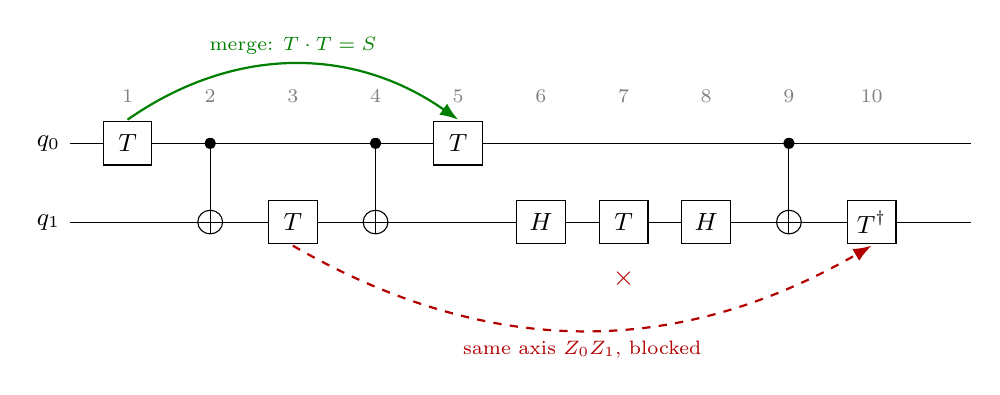
\begin{tikzpicture}[x=1.05cm,y=1cm, every node/.style={font=\small}]
  % wires
  \draw (0.3,1) node[left] {$q_0$} -- (11.2,1);
  \draw (0.3,0) node[left] {$q_1$} -- (11.2,0);
  % gate helper
  \newcommand{\gbox}[3]{\node[draw,fill=white,minimum width=0.62cm,minimum height=0.55cm] at (#1,#2) {#3};}
  \newcommand{\cnot}[1]{\fill (#1,1) circle (0.07); \draw (#1,1) -- (#1,-0.15); \draw (#1,0) circle (0.15);}
  \gbox{1}{1}{$T$}
  \cnot{2}
  \gbox{3}{0}{$T$}
  \cnot{4}
  \gbox{5}{1}{$T$}
  \gbox{6}{0}{$H$}
  \gbox{7}{0}{$T$}
  \gbox{8}{0}{$H$}
  \cnot{9}
  \gbox{10}{0}{$T^\dagger$}
  % numbers
  \foreach \k in {1,...,10} { \node[gray] at (\k,1.6) {\scriptsize \k}; }
  % merge arc 1 -> 5
  \draw[-{Latex}, thick, green!50!black] (1,1.3) to[out=35,in=145] node[above] {\scriptsize merge: $T\cdot T = S$} (5,1.3);
  % blocked arc 3 -> 10
  \draw[-{Latex}, thick, red!70!black, dashed] (3,-0.3) to[out=-30,in=-150] node[below,pos=0.5] {\scriptsize same axis $Z_0Z_1$, blocked} (10,-0.3);
  \node[red!70!black, font=\bfseries] at (7,-0.72) {$\times$};
\end{tikzpicture}
\caption{A circuit for Algorithm~\ref{alg:pfr}. The $T$ at gate 1 slides past the
$\gate{CX}$--$T$--$\gate{CX}$ block, whose rotation acts on $Z_0Z_1$ and commutes with
$Z_0$, and merges into gate 5 as an $\gate S$. The $T$ at gate 3 and the $T\adj$ at
gate 10 share the axis $Z_0Z_1$. The $T$ at gate 7 has axis $X_1$, which anticommutes with
$Z_0Z_1$, so they cannot meet.}
\label{fig:pfr}
\end{figure}

\begin{table}[h]
\centering
\renewcommand{\arraystretch}{1.25}
\small
\begin{tabular}{rllllp{6.1cm}}
\toprule
 & gate & $x_0,\ z_0$ & $x_1,\ z_1$ & axis & action \\
\midrule
  & start & $X_0,\ Z_0$ & $X_1,\ Z_1$ & & \\
1 & $T_0$ & $X_0,\ Z_0$ & $X_1,\ Z_1$ & $+Z_0$ & no earlier axis $Z_0$: record $e_1$ \\
2 & $\gate{CX}_{0,1}$ & $X_0X_1,\ Z_0$ & $X_1,\ Z_0Z_1$ & & $x_0 \gets x_0x_1$, \ $z_1 \gets z_0z_1$ \\
3 & $T_1$ & & & $+Z_0Z_1$ & no earlier axis $Z_0Z_1$: record $e_2$ \\
4 & $\gate{CX}_{0,1}$ & $X_0,\ Z_0$ & $X_1,\ Z_1$ & & the rows return \\
5 & $T_0$ & & & $+Z_0$ & candidate $e_1$. After $e_1$: $e_2 = Z_0Z_1$ commutes with $Z_0$. \textbf{Merge}: $\tfrac{\pi}{4}+\tfrac{\pi}{4} = \tfrac{\pi}{2}$. Delete gate 1, emit $\gate S$ at 5, kill $e_1$, and apply $\gate S$ to the frame. \\
  & ($\gate S$) & $-\tY_0,\ Z_0$ & & & $x_0 \gets -i\,x_0z_0 = -i\,X_0Z_0 = -Y_0$ \\
6 & $\gate H_1$ & & $Z_1,\ X_1$ & & swap $x_1, z_1$ \\
7 & $T_1$ & & & $+X_1$ & no earlier axis $X_1$: record $e_3$ \\
8 & $\gate H_1$ & & $X_1,\ Z_1$ & & swap back \\
9 & $\gate{CX}_{0,1}$ & $-Y_0X_1,\ Z_0$ & $X_1,\ Z_0Z_1$ & & \\
10 & $T\adj_1$ & & & $+Z_0Z_1$ & candidate $e_2$. After $e_2$: $e_3 = X_1$ \emph{anticommutes} with $Z_0Z_1$. \textbf{Blocked}: record $e_4$. \\
\bottomrule
\end{tabular}
\caption{The scan of Figure~\ref{fig:pfr}. Empty cells are unchanged.}
\label{tab:pfr-trace}
\end{table}

The output is the circuit with gate 1 deleted and gate 5 replaced by $\gate S$. It has
three $T$ gates instead of five; this is exactly what \texttt{tzap --passes PhaseFoldPauli}
produces. Without gates 6--8 the $T$ at gate 3 and the $T\adj$ at gate 10 would merge and
cancel as well.

\subsection{Relation to the abstraction}

\begin{itemize}[nosep]
  \item \emph{The frame.} The frame is the tableau of Section~2, with the transformer
  of Table~\ref{tab:rows}.
  \item \emph{The history.} The live events are its axes, each annotated with an angle, with
  blockers added for Toffolis, measurements and resets.
  \item \emph{The fold rule.} ``Same axis, and every axis recorded between them commutes
  with it'' is the fact $(s Z_q, Z_{q'})$ of the segment's abstract state
  (Lemma~\ref{lem:scan-check}). By Theorem~\ref{thm:fold}, that single fact licenses the
  merge.
  \item \emph{Order.} The history is ordered only so that one global list serves every
  segment. The segment's own axes are a contiguous slice of it, conjugated by $C_i$.
\end{itemize}
Theorem~\ref{thm:fold} is proved in Lean (\texttt{FoldRule.lean}), with phase-exact
rotations $\mathrm{diag}(1, e^{i\pi\theta})$ in place of $R_P(\theta)$. For the sign $-$,
the two versions differ by the global phase $e^{i\pi\theta}$. Corollary~\ref{cor:fold-programs}
and Lemma~\ref{lem:scan-check} are argued on paper only.

\section{Making the scan fast}\label{sec:fast}

Algorithm~\ref{alg:pfr} as written costs $O(rn)$ per rotation: it compares a new axis with
every earlier event, and it tests commutation against every event since the candidate. On
circuits with $10^7$ gates this is far too slow. This section describes how the Rust pass
gets its speed, in the order the pieces matter. Every optimization here either answers the
same question faster or refuses a fold. None of them can authorize a rewrite that
Algorithm~\ref{alg:pfr} would reject.

\subsection{Finding the candidate: fingerprints}

\paragraph{Fingerprints.}
Each generator $X_q$, $Z_q$ gets a random 128-bit label $\lambda(X_q)$, $\lambda(Z_q)$. The
\emph{fingerprint} of a Pauli string, ignoring its sign, is the XOR of the labels of the
generators it contains, with $Y_q$ counting as both $X_q$ and $Z_q$:
\[
  f(\tX^u \tZ^w) = \bigoplus_{u_q = 1} \lambda(X_q) \;\oplus\; \bigoplus_{w_q = 1} \lambda(Z_q).
\]
Multiplying Pauli strings XORs their bit vectors, so $f(PQ) = f(P) \oplus f(Q)$. Every row
update of Table~\ref{tab:rows} is a swap, a sign change, or a product of two rows. So a
second, \emph{sketch} frame can hold the fingerprints of the rows and update them with the
same pattern, at $O(1)$ per gate instead of $O(n/64)$.

\paragraph{The candidate index.}
A hash map sends each fingerprint to its newest event, and each event links to the
previous event with the same fingerprint. The candidate search on line~7 is then one
lookup, followed by exact axis comparisons along that chain until one matches. Two cases
remain:
\begin{itemize}[nosep]
  \item \emph{Collisions.} Different axes collide with probability $2^{-128}$. A collision
  only costs a wasted comparison, because the exact axes decide.
  \item \emph{Dead links.} Links to dead events are skipped and then compressed, so a long
  run of folds on one axis does not make later lookups walk it again.
\end{itemize}
The randomness therefore affects only speed. The output is deterministic.

\paragraph{The pre-check.}
Before building anything, the pass runs the sketch frame alone and records the
fingerprint of every rotation's axis. If no fingerprint repeats, no two rotations share an
axis, and the circuit is returned unchanged without ever building the exact frame.

\subsection{Checking commutation: support lists}

\paragraph{Support lists.}
Two Pauli strings can anticommute only on a qubit where both act. For each qubit block $b$
(the qubits are split into at most 64 blocks), the pass keeps the list of events whose
axis acts on $b$, in increasing order. To check line~8, it looks at the lists of the blocks
where $A$ acts. In each one, it binary-searches for the first event after the candidate
and tests the events from there.

\paragraph{Test each event once.}
An event that shares several blocks with $A$ appears in several of these lists. Each event
records its \emph{signature}, the 64-bit mask of blocks it acts on. It is tested only in
the list of the lowest block it shares with $A$, that is, when
$\mathrm{ctz}(\mathrm{sig}_e \wedge \mathrm{sig}_A)$ is the current block.

\paragraph{Liveness without indirection.}
The scan needs each event's liveness and axis. Liveness is kept in a separate bitset, one
bit per event. Axes are stored contiguously, $2\lceil n/64\rceil$ words each, so event
$e$'s axis starts at a fixed offset. The inner loop therefore reads two small arrays
instead of following a pointer into a large event record.

\subsection{The dominant cost: folded rotations}

\paragraph{The problem.}
On the large cobble circuits, 98\% of the $T$ gates fold away. Their events die, but their
ids stayed in the support lists. We measured the lists on \texttt{ols-ridge-d24} (20M gates,
28 qubits):
\begin{itemize}[nosep]
  \item the commutation checks visited $6.2 \times 10^9$ list entries;
  \item 98\% of those entries were dead;
  \item the check took 88\% of the pass.
\end{itemize}
Most of the visits came from \emph{blocked} attempts. A rotation whose axis last appeared
tens of thousands of events earlier has a long window. The scan then walks thousands of
dead entries before it meets the live event that blocks the fold.

\paragraph{Compaction.}
Each list keeps a count of its dead entries. When a rotation dies, the count goes up in
each of its lists. A list is compacted, keeping only live ids and preserving their order,
once a quarter of it is dead. Each compaction is linear in the list, and at least a
quarter of its entries died since the previous one, so the cost is $O(1)$ amortized per
death. On \texttt{ols-ridge-d24} this cut the visits from $6.2 \times 10^9$ to
$3.6 \times 10^8$, and the output did not change.

\paragraph{Scan order does not help.}
The verdict, whether some live event in the window anticommutes with $A$, does not depend
on the order of the scan. We tried scanning newest first, and the result depended on the
circuit:
\begin{itemize}[nosep]
  \item on some circuits it was 2$\times$ faster;
  \item on the \texttt{ols-ridge} family it was 3.5$\times$ slower, because there the
  blockers sit near the old end of the window.
\end{itemize}
Alternating between the two ends gave middling results everywhere. The scan stays
oldest-first.

\subsection{Bit-sliced lists}

The remaining cost is testing one event at a time. For circuits with at most 32 qubits, an
axis is one X word and one Z word. Two axes $P = (x, z)$ and $Q = (x', z')$ anticommute
exactly when
\[
  \omega(P, Q) \;=\; \mathrm{popcount}\big((x \wedge z') \oplus (z \wedge x')\big) \bmod 2 \;=\; 1 .
\]
Its terms can be regrouped by qubit, so the test runs on 64 events at once.

\paragraph{The layout.}
Each qubit's list is stored in blocks of 64 entries. Entry $i$ of a block owns bit $i$ of
every mask in that block. A block holds, for each qubit $p$:
\begin{itemize}[nosep]
  \item $\mathrm{X}_p$, the mask of entries whose axis has $X$ or $Y$ on $p$;
  \item $\mathrm{Z}_p$, the mask of entries with $Z$ or $Y$ on $p$;
\end{itemize}
and one mask $\mathrm{L}$ of live entries.

\paragraph{The test.}
Anticommutation with $A = (a_x, a_z)$ is the parity, over the qubits $p$ of $A$'s support,
of ``$A$ has $X$ on $p$ and the entry has $Z$ on $p$'' plus ``$A$ has $Z$ on $p$ and the
entry has $X$ on $p$''. For all 64 entries at once, that is
\[
  \mathrm{hit} \;=\; \Big( \bigoplus_{p \,:\, a_x(p) = 1} \mathrm{Z}_p \;\;\oplus\;
  \bigoplus_{p \,:\, a_z(p) = 1} \mathrm{X}_p \Big) \wedge \mathrm{L} .
\]
Any set bit is a live anticommuting event, so the fold is blocked. A block costs
$\mathrm{wt}(A)$ word XORs instead of 64 separate tests. The per-entry storage is small:
$2n$ bits of masks plus a 32-bit id, about 11 bytes for $n = 28$.

\begin{example}[One block]
Take two qubits and a block with four entries,
$e_0 = Z_0Z_1$, $e_1 = X_1$, $e_2 = X_0X_1$ and $e_3 = Y_0$, with $e_1$ dead. Writing
masks as $e_3e_2e_1e_0$:
\[
  \mathrm{X}_0 = 1100,\quad \mathrm{Z}_0 = 1001,\quad \mathrm{X}_1 = 0110,\quad
  \mathrm{Z}_1 = 0001,\quad \mathrm{L} = 1101 .
\]
\begin{itemize}[nosep]
  \item For $A = Z_1$, only $a_z(1) = 1$, so $\mathrm{hit} = \mathrm{X}_1 \wedge \mathrm{L}
  = 0100$. That is $e_2 = X_0X_1$, the only live entry that anticommutes with $Z_1$. The
  entry $e_1 = X_1$ also anticommutes, but it is dead.
  \item For $A = X_0Z_1$, $\mathrm{Z}_0 \oplus \mathrm{X}_1 = 1111$: every entry
  anticommutes with $X_0Z_1$, and $\mathrm{hit} = 1101$.
\end{itemize}
\end{example}

\paragraph{Updates.}
\begin{itemize}[nosep]
  \item \emph{A new event} with support $w$ goes into $w$ lists and sets up to $w$ mask bits
  in each, so recording it costs $O(w^2)$ rather than $O(w)$.
  \item \emph{A death} clears one bit of $\mathrm{L}$ in each of the event's lists. Its
  position there is found by a galloping search from the end, because rotations usually
  fold soon after they are recorded.
  \item \emph{Compaction.} A list is rebuilt from its live entries once half of it is dead.
\end{itemize}

\paragraph{When to use it.}
Scans get cheaper and insertions get more expensive. The trade pays off when fold attempts
scan long windows, as on the cobble circuits, and loses when axes are dense and few
rotations fold, as on QFT. On 50-qubit QFT, bit-slicing made the pass 2.2$\times$ slower.
The pass therefore uses bit-sliced lists up to 32 qubits and the scalar lists above that.
A test checks that the two kinds reach the same verdicts: with an unbounded budget, they
produce identical rewrites on 600 random circuits with measurements, CCX and CCZ.

\subsection{The budget}

Each fold attempt gets a budget of $2^{16}$ steps. The candidate search and the
commutation check share it.
\begin{itemize}[nosep]
  \item \emph{Candidate search:} one step per live chain entry compared.
  \item \emph{Scalar lists:} one step per list entry visited.
  \item \emph{Bit-sliced lists:} one step per live entry in each block scanned.
\end{itemize}
An attempt that runs out counts as blocked. The rotation is then recorded as a new event,
and the scan goes on. This bounds the pass by $O(m + r \cdot 2^{16})$. It is sound, because
it only refuses folds.

Once the scan was fast, the budget stopped mattering. Across 63 benchmark circuits:

\begin{center}
\small
\begin{tabular}{@{}lrrr@{}}
\toprule
budget per attempt & pass time & rotations left & lost folds vs.\ $2^{20}$ \\
\midrule
$2^{8}$ & 6.9 s & 13{,}220{,}606 & 10{,}823{,}123 \\
$2^{10}$ & 5.8 s & 2{,}402{,}329 & 4{,}846 \\
$2^{12}$ & 5.9 s & 2{,}398{,}399 & 916 \\
$2^{16}$ & 6.1 s & 2{,}397{,}821 & 338 \\
$2^{20}$ & 6.2 s & 2{,}397{,}483 & 0 \\
\bottomrule
\end{tabular}
\end{center}

Below about $2^{10}$ folds collapse, and the pass even gets slower: unfolded rotations stay
live and lengthen every list. Above it, the time moves by less than 7\%.

\subsection{Results}

These timings are for the pass alone: one thread, on the whole circuit, timed in process
on the same parsed input. \texttt{PhaseFoldRand} is shown for scale.

\begin{center}
\small
\begin{tabular}{@{}lrrrrr@{}}
\toprule
circuit & gates & original & compaction & all & \texttt{PhaseFoldRand} \\
\midrule
\texttt{ols-ridge-d24} & 19.8M & 3.73 s & 3.01 s & 2.42 s & 0.56 s \\
\texttt{hamiltonian-n18} & 10.6M & 4.97 s & 2.27 s & 0.97 s & 0.24 s \\
\texttt{chebyshev-n36} & 10.4M & 2.32 s & 1.50 s & 0.99 s & 0.25 s \\
\texttt{spectral-n29} & 10.2M & 11.69 s & 6.54 s & 1.14 s & 0.26 s \\
all 63 circuits & & 23.6 s & 13.8 s & 6.2 s & 1.5 s \\
\bottomrule
\end{tabular}
\end{center}

Over all 63 circuits the pass is 3.8$\times$ faster than it was. It still costs about four
times \texttt{PhaseFoldRand}, but it leaves 2.4M rotations to \texttt{PhaseFoldRand}'s
19.4M. On the 97-circuit corpus, the CLI output is byte-identical on 93 circuits. The other
4 have a few more folds, from attempts that used to exhaust the budget on dead entries.

The CLI splits a circuit into chunks and runs them in parallel. Each chunk then has a short
history, so there the gain is larger. On \texttt{ols-ridge-d24}, compaction alone took the
pass itself from about 5 s to about 0.1 s, against a trivial pass on the same file. The price is that chunking gives up the folds that would cross a
chunk boundary.

What remains is spread out: the commutation check, deaths, the candidate hash lookup, and
the frame updates each take 10--30\% of the pass. A further step would choose bit-sliced
lists by average axis density rather than by qubit count, to recover QFT's 20- and
30-qubit cases, which are now 0.75--0.83$\times$ their old speed.

\section{Comparison with Amy and Lunderville's relational analyses}\label{sec:al}

Amy and Lunderville (POPL 2025) recast phase folding as a \emph{relational analysis}. A
program is abstracted by the classical transitions it can make: the pairs of basis states
$(x, x')$ with $\langle x' | U | x\rangle \neq 0$. They give two domains for these
transitions:
\begin{itemize}[nosep]
  \item $\mathrm{PF}_{\mathrm{Aff}}$, affine relations over $\mathbb{F}_2$;
  \item $\mathrm{PF}_{\mathrm{Pol}}$, polynomial relations, as ideals with Gr\"obner bases.
\end{itemize}
They also give a way to strengthen either one by rewriting the program's path sum
(\emph{Strengthen}).

\paragraph{Scope of the Lean comparisons.}
Lean's \texttt{StateFold} and \texttt{Strengthen} are \emph{restricted} models of these
analyses. They keep only facts $Z_q \mapsto \pm Z_{q'}$, not general transition relations.
Their witnessed constraints are taken on the final path sum only, not accumulated as in
Algorithm~2, and the degree bound $d$ limits only HH substitutions. Separations in which the
path-sum analysis proves more transfer to the full domain. \texttt{Alpha.lean} also defines
the paper's path-sum abstraction $\alpha = \exists Y.\langle X' \oplus f(X,Y)\rangle$
(their Definition~17) and Algorithm~1's rewriting. It proves soundness and monotonicity
(their Propositions~18 and~21), and it proves both separations against $\alpha$ itself
(\texttt{alpha\_pauli\_incomparable}). Only Strengthen's accumulated ideal is still
modeled in restricted form.

\paragraph{Domain versus analysis.}
A separation can come from what a domain can \emph{express}, or from what an analysis
manages to \emph{compute}.
\begin{itemize}[nosep]
  \item \emph{Expressiveness.} Every affine relation is a $Z$-type Pauli fact, so the
  tableau's facts cover affine relations and add $X$- and $Y$-type facts. Polynomial
  relations and Pauli facts are incomparable: $x' = x \oplus ab$ is not a Pauli fact, and
  $X \mapsto X$ is not a relation on the computational basis.
  \item \emph{What is computed.} The relational analyses compute their abstraction by
  rewriting with a fixed rule set, which can fall short of the best abstraction
  $\alpha(U)$.
\end{itemize} This section compares those analyses with the tableau domain. It
states what each one records and where each one is more precise, with an example for
every separation.

\subsection{What each analysis records}

\begin{table}[h]
\centering
\small
\renewcommand{\arraystretch}{1.25}
\begin{tabular}{@{}p{2.3cm}p{3.9cm}p{3.6cm}p{4.2cm}@{}}
\toprule
 & $\mathrm{PF}_{\mathrm{Aff}}$ & $\mathrm{PF}_{\mathrm{Pol}}$ (+ Strengthen) & tableau (this note) \\
\midrule
state & affine relations among the outputs $x'$, inputs $x$ and path variables $y$ & polynomial
relations among $x', x, y$ & rows $x_q, z_q$ (the Clifford part) and axes \\
facts & $x'_S = x_T \oplus c$ & $f(x', x) = 0$ & $U\,\back(P)\,U\adj = P$ for all $P$ with
$\back(P)$ commuting with the axes \\
$\gate H$ & fresh variable $y$ ($x'_q$ is forgotten) & fresh variable, removed later by
path-sum rewriting & exact: swap the rows \\
$\gate T$, $R_Z$ & a phase term on a linear function; the relation is unchanged & the same &
records the axis $z_q$ \\
$\gate{CCX}$ & target forgotten & exact: $x'_t = x_t \oplus x_ax_b$ & seven axes \\
measure & $x'_q = x_q$ & $x'_q = x_q$ & the axis $z_q$ \\
reset & $x'_q = 0$ (a state fact) & $x'_q = 0$ & the axes $z_q, x_q$ (no state fact) \\
join & affine hull & product of ideals & per-row, or disjunctive (Section~\ref{sec:disj}) \\
merge rule & same linear function modulo the relation (their Prop.~9) & the same, modulo the
ideal & Theorem~\ref{thm:fold} \\
\bottomrule
\end{tabular}
\caption{The three analyses side by side.}
\label{tab:al}
\end{table}

\paragraph{The bridge: relations are $Z$-facts.}
An affine relation says the parity of the outputs on a set $S$ equals the parity of the
inputs on a set $T$, plus a constant $c$. This is exactly the Pauli fact
\[
  U\, Z_T\, U\adj = (-1)^c Z_S ,
\]
where $Z_T = \prod_{q \in T} Z_q$. Lean proves both directions: a relation gives the fact
(\texttt{rel\_pauliFact}), and a unitary with the fact satisfies the relation on its whole
support (\texttt{support\_of\_zfact}).

So the affine domain speaks only about \emph{$Z$-type} facts, meaning facts about the
computational basis. The tableau speaks about every Pauli, and it treats $\gate H$ exactly.
Their merge rule, Proposition~9, requires $x'_j = x_i$ on every transition of the segment.
That is Theorem~\ref{thm:fold} with the segment fact $(Z_i, Z_j)$. For straight-line
circuits, this gives:

\begin{theorem}[Tableau refines affine, straight-line; Lean]\label{thm:tab-aff}
For every Clifford+$T$ circuit $c$, $\gam(\abs{c}) \subseteq \gam_{\mathrm{Aff}}(c)$, and the
inclusion is strict on $\gate H\,\gate H$.
\end{theorem}

Here $\gam_{\mathrm{Aff}}$ is the affine analysis without path-sum rewriting, with $\gate H$
as a fresh variable. In Lean these are \texttt{affGamma} and
\texttt{tableau\_refines\_aff\_strict}. Path-sum
rewriting and non-linear relations add facts that the tableau cannot express, and there the
domains become incomparable (Section~\ref{sec:al-ex}).

\subsection{Examples}\label{sec:al-ex}

Throughout, ``folds'' means the analysis proves the fact that Theorem~\ref{thm:fold} (or
their Proposition~9) needs.

\paragraph{Tool check.}
The straight-line examples were run through both tools.
\begin{itemize}[nosep]
  \item \emph{tzap.} \texttt{tzap --passes PhaseFoldPauli}, with each output checked for
  equivalence by simulation.
  \item \emph{Feynman.} \texttt{feynopt -verify}, at commit \texttt{4c4c488}, through its
  \texttt{.qc} frontend. Every output verified. The QASM2 frontend with
  \texttt{-purecircuit} gives the same counts, and its outputs are equivalent by
  simulation.
\end{itemize}
In the table, \texttt{sf} $d$ is \texttt{-statefold} $d$, and $d = 0$ means unbounded.

\begin{center}
\small
\begin{tabular}{@{}lcccccc@{}}
\toprule
example & $T$ in & tzap & \texttt{-phasefold} & \texttt{sf 1} (affine) &
\texttt{sf 2} & \texttt{sf 0} \\
\midrule
\ref{ex:al-hframe} $\gate H$ frame & 2 & 0 & 2 & 0 & 0 & 0 \\
\ref{ex:al-pauli} Clifford segment & 2 & 0 & 2 & 2 & 2 & 2 \\
\ref{ex:al-toffoli} relative Toffoli & 11 & 11 & 11 & 11 & 9 & 9 \\
\bottomrule
\end{tabular}
\end{center}

Feynman's \texttt{-apf} and \texttt{-ppf} pipelines also fold
Example~\ref{ex:al-pauli} to 0. They include Feynman's own Pauli-folding pass
(\texttt{Paulifold 1}), which is not part of the relational analyses. The loop and reset
examples, and the tableau's entries for them, are hand analyses: tzap reads no loops, and
Feynman's verifier covers only \texttt{.qc} circuits. The QASM2 frontend gives the same
counts with \texttt{-purecircuit}. Without that flag it assumes every qubit starts in
$|0\rangle$, a different semantics under which, for example, a leading $T$ is removed.

\begin{example}[An $\gate H$ frame]
\label{ex:al-hframe}
Take $\gate H_a\ \gate T_a\ \gate H_a\ \gate{CX}_{b,a}\ \gate H_a\ \gate T_a\ \gate H_a$.
\begin{itemize}[nosep]
  \item \emph{Tableau.} Both $T$ gates have axis $X_a$, since $\gate{CX}_{b,a}$ does not
  change $x_a$. So they merge into an $\gate S$, and 2 $T$ become 0.
  \item \emph{Affine.} The four $\gate H$ gates introduce $y_1, \dots, y_4$. The $T$ gates
  act on $y_1$ and $y_3$, and no relation links them, so nothing folds.
  \item \emph{Path sums.} The phase contains $y_2(y_1 \oplus y_3)$. Summing out $y_2$ (the
  (H) rule) witnesses $y_1 = y_3$, so Strengthen folds too.
\end{itemize}
The tableau gets this fold directly from the row update for $\gate H$, with no rewriting.
\end{example}

\begin{example}[A Clifford segment]\label{ex:al-pauli}
Take $\gate T_1\ \gate{CX}_{0,1}\ \gate H_0\ \gate H_1\ \gate{CX}_{1,0}\ \gate H_1\ \gate T\adj_1$.
\begin{itemize}[nosep]
  \item \emph{Tableau.} The segment between the rotations is Clifford and maps $Z_1$ to
  $Z_1$. So the $T$ and $T\adj$ cancel, and 2 $T$ become 0.
  \item \emph{Path sums.} Both output wires mention every path variable, so neither rewrite
  rule applies, and there is no witness. The wire map is onto, so $\alpha$ is $\top$,
  and nothing folds (\texttt{alpha\_cexMid}). This is a limit of the rules, not of the
  domain. The exact $\alpha(U)$ contains $x'_1 = x_1$. Renaming the $q_0$ wire
  $u = y_0 \oplus y_1$ turns the phase into $x_0u + y_1(x_1 \oplus y_2)$. An (H) step on
  $y_1$ then gives $y_2 = x_1$, and Feynman's \texttt{-cxcz} preprocessing finds exactly
  this.
  \item \emph{Affine.} The $\gate H$ gates forget the wires.
\end{itemize}
So the tableau is not below Algorithm~1 as the circuit is written. This is a separation of
analyses, not of domains.
\end{example}

\begin{example}[A relative-phase Toffoli]
\label{ex:al-toffoli}
Take the 21-gate circuit $\gate T_0\ G\ \gate T\adj_0\ G\ \gate T_0$ (in Lean,
\texttt{DegreeTwo.lean}), where $G$ is a relative-phase Toffoli with target $0$.
\begin{itemize}[nosep]
  \item \emph{Path sums, degree 2.} The analysis proves that the outer axis $Z_0$ returns
  unchanged (\texttt{midE\_ssubset}), because $G$ computes and then uncomputes
  $x_0 \oplus x_1x_2$.
  \item \emph{Tableau.} It records axes inside $G$ that anticommute with $Z_0$, so the outer
  $T$ gates are blocked, and all 11 remain.
\end{itemize}
The missing ingredient is a \emph{non-linear} classical function. The tableau sees $G$ only
through its axes.
\end{example}

\begin{example}[State knowledge: \emph{Reset-simple}]\label{ex:al-reset}
Take $\gate T_a$; $\mathsf{reset}\ a$; $\gate T_a$.
\begin{itemize}[nosep]
  \item \emph{Affine.} The reset sets $x'_a = 0$, so the second $T$ has phase condition 0
  and is deleted, leaving 1 $T$.
  \item \emph{Tableau.} The reset only adds the axes $z_a$ and $x_a$, so both $T$ remain.
\end{itemize}
Recovering this needs stabilizer facts $P\cdot K = K$ about the current state, an extension
of the domain not developed here. \emph{Loop-nested} fails for the same reason: its
$\gate T_a$ acts on a qubit that was reset before the loop.
\end{example}

\begin{example}[A loop in an $\gate H$ frame]
\label{ex:al-loop-h}
Take $\gate T_a$; $\textbf{while}\ \star\ \textbf{do}\ (\gate H_a\ \gate{CX}_{b,a}\
\gate H_a)$; $\gate T\adj_a$. The body is $\gate{CZ}_{a,b}$ written with $\gate H$ gates.
\begin{itemize}[nosep]
  \item \emph{Tableau.} The body maps $z_a \mapsto Z_a$ and $z_b \mapsto Z_b$. The per-row
  join with the identity keeps both $z$ rows and forgets the $x$ rows. So the $T$ and
  $T\adj$ cancel.
  \item \emph{Affine.} The body's $\gate H$ gates forget $x_a$, so the loop summary has no
  relation on $a$, and nothing folds.
  \item \emph{Path sums.} Summarizing the body by path-sum rewriting recovers
  $x'_a = x_a$, so $\mathrm{PF}_{\mathrm{Pol}}$ with Strengthen folds too.
\end{itemize}
\end{example}

\begin{example}[An $S_4$ loop: the affine hull beats both joins]\label{ex:al-perm}
Let the body of $\textbf{while}\ \star$ be a nondeterministic choice between
$\mathsf{SWAP}_{a,b}$ and the 4-cycle $(a\,b\,c\,d)$. Around the loop, place a $T$ and a
$T\adj$ on the parity $x_a \oplus x_b \oplus x_c \oplus x_d$, each conjugated by a CNOT
ladder.
\begin{itemize}[nosep]
  \item \emph{Affine.} Every permutation preserves the total parity, so the affine hull of
  the reachable permutations keeps $x'_a\oplus x'_b\oplus x'_c\oplus x'_d =
  x_a\oplus x_b\oplus x_c\oplus x_d$, and the rotations fold.
  \item \emph{Per-row join.} It forgets every row after one iteration, giving $\top$.
  \item \emph{Disjunctive join.} It must keep all 24 permutations of $S_4$. It exceeds
  $\mathit{bound} = 8$ and collapses to the per-row join, giving $\top$.
\end{itemize}
A join that keeps the \emph{subgroup} of Paulis on which two states agree,
$\{P : \back_1(P) = \back_2(P)\}$, would keep $Z_aZ_bZ_cZ_d$ here. It is computable by
linear algebra over $\mathbb{F}_2$, and it would subsume the affine hull on $Z$-type facts.
We have not built it.
\end{example}

\subsection{Summary}

\begin{table}[h]
\centering
\small
\renewcommand{\arraystretch}{1.2}
\begin{tabular}{@{}lccccc@{}}
\toprule
example & plain affine & path sums / Pol & tableau, per-row & tableau, disjunctive \\
\midrule
\ref{ex:al-hframe} $\gate H$ frame & -- & \checkmark & \checkmark & \checkmark \\
\ref{ex:al-pauli} Clifford segment & -- & -- & \checkmark & \checkmark \\
\ref{ex:al-toffoli} relative Toffoli & -- & \checkmark\ ($d \ge 2$) & -- & -- \\
\ref{ex:al-reset} reset & \checkmark & \checkmark & -- & -- \\
\ref{ex:al-loop-h} loop in $\gate H$ frame & -- & \checkmark & \checkmark & \checkmark \\
Loop-swap (Ex.~\ref{ex:swap-loop}) & \checkmark & \checkmark & -- & \checkmark \\
\ref{ex:al-perm} $S_4$ loop & \checkmark & \checkmark & -- & -- \\
\bottomrule
\end{tabular}
\caption{Which analyses fold each example. \checkmark: the fold is proved; --: it is not.}
\label{tab:al-summary}
\end{table}

\paragraph{Table 1 of Amy and Lunderville.}
The paper's numbers, next to the tableau domain's analyzed by hand with the joins of
Section~\ref{sec:loops}:

\begin{center}
\small
\begin{tabular}{@{}lrrrrl@{}}
\toprule
program & $T$ in & $\mathrm{PF}_{\mathrm{Aff}}$ & $\mathrm{PF}_{\mathrm{Pol}}$ & tableau & reason for a gap \\
\midrule
If-simple & 2 & 0 & 0 & 0 & \\
Loop-simple & 2 & 0 & 0 & 0 & \\
Loop-h & 2 & 0 & 0 & 0 & \\
Loop-swap & 2 & 0 & 0 & 0 & disjunctive join (per-row: 2) \\
Loop-null & 4 & 2 & 2 & 2 & \\
Grover (per iteration) & 1736 & 1472 & timeout & 1472 & \\
RUS & 16 & 10 & 8 & 10 & non-linear (Toffoli) \\
Loop-nonlinear & 30 & 18 & 0 & 18 & non-linear invariant \\
Loop-nested & 3 & 2 & 2 & 3 & reset: state fact \\
Reset-simple & 2 & 1 & 1 & 2 & reset: state fact \\
\bottomrule
\end{tabular}
\end{center}

The tableau matches $\mathrm{PF}_{\mathrm{Aff}}$ except on the two programs that need state
facts from a reset. It trails $\mathrm{PF}_{\mathrm{Pol}}$ on the two that need non-linear
relations. Its advantages are elsewhere, in Clifford segments with $\gate H$ gates
(Examples~\ref{ex:al-hframe}, \ref{ex:al-pauli} and~\ref{ex:al-loop-h}), which Table~1 does
not exercise.

\paragraph{Where the precision comes from.}
\begin{itemize}[nosep]
  \item \emph{Tableau.} It is exact on every Clifford, $\gate H$ included, and it proves
  $X$- and $Y$-type facts.
  \item \emph{Relational analyses.}
  \begin{itemize}[nosep]
    \item \emph{State facts:} constants after a reset, and ancillas known to be $|0\rangle$.
    \item \emph{Non-linear classical functions:} Toffoli gates and polynomial loop
    invariants.
    \item \emph{Interference found by path-sum rewriting:} the (H) rule on $T$-free
    variables.
  \end{itemize}
\end{itemize}
The two kinds of analysis are sound independently, so their facts can be combined: a merge
is valid if either analysis proves the segment fact. The two gaps in Table~1 are exactly the
stabilizer extension and a non-linear component.

\appendix
\section{Correspondence with the Lean formalization}\label{app:lean}

Everything above is proved in Lean, except Proposition~\ref{prop:char}, its corollary,
Lemma~\ref{lem:products}, the examples before Section~\ref{sec:loops}, and
Section~\ref{sec:rust} apart from Theorem~\ref{thm:fold}, which are argued on paper only. The loop examples of Section~\ref{sec:loops} are checked in Lean by evaluation.
The development is in the files
\begin{center}\texttt{lean-paulifold/PauliFold/Tableau.lean}, \quad \texttt{Join.lean}, \quad
\texttt{Disjunctive.lean}, \quad \texttt{FoldRule.lean},\end{center}
and its proofs are against the gate matrices of \texttt{TzapLean.gateUnitary}.

\begin{center}
\renewcommand{\arraystretch}{1.2}
\begin{tabular}{ll}
\toprule
this note & Lean \\
\midrule
Pauli strings $\Pauli$, product, matrix & \texttt{PP}, \texttt{PP.mul}, \texttt{PP.toMatrix} \\
Lemma~\ref{lem:pauli-product} (product) & \texttt{PP.toMatrix\_mul} \\
Lemma~\ref{lem:commute} (commutation) & \texttt{PP.Comm}, \texttt{PP.Comm.toMatrix} \\
Lemma~\ref{lem:decomp} (decomposition) & \texttt{PP.restrict\_cons}, \texttt{PP.restrict\_all} \\
Lemma~\ref{lem:rot} (rotations) & \texttt{embed1\_diag2}, \texttt{rotation\_decomp} \\
abstract states, $\sigma_0$ & \texttt{Tab}, \texttt{Tab.init} \\
pull-back $\back_\sigma$, Lemma~\ref{lem:back} & \texttt{Tab.back}, \texttt{Tab.back\_ok} \\
transformers, abstract semantics & \texttt{Tab.step}, \texttt{Tab.run} \\
Table~\ref{tab:rows} (the transformer) & \texttt{Tab.step} \\
Lemma~\ref{lem:rows} (row updates) & \texttt{Tab.step\_rows}, \texttt{Tab.step\_rows\_back} \\
right column of Table~\ref{tab:rows} & \texttt{pull\_h\_X}, \dots, \texttt{pull\_cz\_Z}, \texttt{pullG\_toMatrix} \\
concretization $\gam$ & \texttt{Tab.gamma} \\
invariant, Lemmas~\ref{lem:inv-init}--\ref{lem:inv-run} & \texttt{Tab.Inv}, \texttt{Tab.inv\_init}, \texttt{Tab.inv\_step}, \texttt{Tab.inv\_run} \\
Theorem~\ref{thm:sound} & \texttt{Tab.tableau\_sound}, \texttt{Tab.circ\_mem\_gamma} \\
partial states, completions & \texttt{PTab}, \texttt{PTab.Extends} (\texttt{Join.lean}) \\
Lemma~\ref{lem:sound-gamma} & \texttt{PTab.back\_extends}, \texttt{gammaA\_of\_sound} \\
Lemma~\ref{lem:partial} & \texttt{stepA\_sound}, \texttt{sound\_of\_le}, \texttt{join\_sound\_left/right} \\
programs, loops & \texttt{Prog}, \texttt{Exec}, \texttt{loopFix}, \texttt{absRun} \\
Theorem~\ref{thm:programs} & \texttt{absRun\_sound}, \texttt{program\_sound} \\
loop examples & \texttt{loopSimple\_Z}, \texttt{loopH\_Z}, \texttt{loopSwap} \\
disjunctive states & \texttt{DAbs}, \texttt{joinD} (\texttt{Disjunctive.lean}) \\
Theorem~\ref{thm:disj} & \texttt{absRunD\_sound}, \texttt{programD\_sound} \\
swap loop & \texttt{loopSwap\_ZZ} \\
Theorem~\ref{thm:fold}, the fact & \texttt{segment\_Z} \\
Theorem~\ref{thm:fold}, slide & \texttt{fold\_pos}, \texttt{fold\_neg} \\
Theorem~\ref{thm:fold}, merge & \texttt{fold\_merge\_pos}, \texttt{fold\_merge\_neg} \\
$\alpha$ (their Def.~17), soundness, Prop.~21 & \texttt{alphaGammaC}, \texttt{alpha\_sound}, \texttt{alphaGamma\_mono} \\
tableau vs.\ $\alpha$ & \texttt{alpha\_pauli\_incomparable}, \texttt{midE\_alpha\_not\_pauli} \\
$\gate T\,m\,\gate T \to m\,\gate S$ (sign $+$), $\to m$ (sign $-$) & \texttt{fold\_t\_t}, \texttt{fold\_t\_t\_neg} \\
\bottomrule
\end{tabular}
\end{center}

In the Lean development:

\begin{itemize}[nosep]
  \item Commutation is \emph{defined} as ``$PQ$ and $QP$ have the same phase''. By
  Lemma~\ref{lem:commute}, this is equivalent to the parity condition.
  \item The Clifford transformer is the explicit update of Table~\ref{tab:rows}. For
  Lemma~\ref{lem:rows}, the right column is computed as $G\adj X_q G$ by the proved forward
  conjugation table of the inverse gate (\texttt{pullG}). Its form is stated gate by gate
  (\texttt{pull\_h\_X}, \dots).
  \item The gate matrices are exactly those of Table~\ref{tab:gates}.
\end{itemize}

\end{document}
